% ====================================================================
%  IEEE TCAD Journal Version — Expanded from MLCAD 2026 Conference Paper
%  Target: 14–16 pages, ≥30% new content
% ====================================================================
\documentclass[journal]{IEEEtran}

% ── packages ─────────────────────────────────────────────────────────
\usepackage[utf8]{inputenc}
\usepackage[T1]{fontenc}
\usepackage{amsmath,amssymb}
\usepackage{graphicx}
\usepackage{booktabs}
\usepackage{multirow}
\usepackage{array}
\usepackage{url}
\usepackage{cite}
\usepackage{xcolor}
\usepackage{balance}
\usepackage{enumitem}
\usepackage{tabularx}
\usepackage{makecell}
\usepackage[hidelinks]{hyperref}

% ── custom column types ──────────────────────────────────────────────
\newcolumntype{C}[1]{>{\centering\arraybackslash}m{#1}}
\newcolumntype{L}[1]{>{\raggedright\arraybackslash}m{#1}}

% ── graphics path ────────────────────────────────────────────────────
\graphicspath{{figures/}}

% ====================================================================
\begin{document}

\title{Building VHDL Processors with Claude Code:\\From 16-Bit to 64-Bit FPU}

\author{George~Teifel,~\IEEEmembership{}
        and~Siamak~Tavakoli%
\thanks{G.~Teifel and S.~Tavakoli are with the Department of Electrical
and Computer Engineering, University of New Mexico, Albuquerque, NM
87131, USA (e-mail: gteifel@unm.edu).}%
\thanks{Manuscript received March 24, 2026.  This paper is an extended
version of a conference paper presented at MLCAD 2026.}}

\markboth{IEEE TRANSACTIONS ON COMPUTER-AIDED DESIGN OF INTEGRATED
CIRCUITS AND SYSTEMS}{Teifel and Tavakoli: Building VHDL Processors
with Claude Code}

\maketitle

% ====================================================================
% ABSTRACT
% ====================================================================
\begin{abstract}
Manual design of register-transfer level (RTL) hardware descriptions
remains a labor-intensive process requiring deep expertise in both
digital logic and synthesis tool chains.  This paper presents a
skill-based methodology for AI-assisted hardware description language
(HDL) generation using Claude Code, an AI coding assistant.  A custom
skill was constructed by merging two community-contributed FPGA design
skills and augmenting them with three capabilities: a simulation-first
test-driven development (TDD) mandate, live documentation retrieval via
Context7 MCP integration, and Vivado version-aware code generation.
Using this skill, six complete RISC-V processor designs were generated
in a single session: three in Verilog and three in VHDL, spanning
16-bit educational cores (RV32I subset), 64-bit integer processors
(RV64I), and a 64-bit processor with a full IEEE~754 double-precision
floating-point unit (RV64IFD).  The most complex design implements 68
instructions across 28 FPU operations in a 5-stage pipeline, consuming
12,969 look-up tables (LUTs) and 18 DSP48E1 slices on a Xilinx Artix-7
XC7A35T.  The simulation-first verification approach identified 10
floating-point bugs in the initial generation and drove a 48\%
reduction in LUT utilization, from approximately 25,000 to 12,969 LUTs.
Formal verification using SystemVerilog Assertions with SymbiYosys
bounded model checking was subsequently integrated, mathematically
proving correctness properties for ALU operations, FPU IEEE~754
special-value handling, pipeline hazard detection, and memory bus
protocols across all three processor variants.  All designs were
verified on a Digilent Basys~3 development board.  Compared to the
conference version, this paper adds a comprehensive comparison with
prior work in AI-assisted HDL generation, detailed timing and resource
analysis, an extended FPU verification coverage matrix, a discussion of
unbounded verification strategies, an expanded related work survey, and
a reproducibility section.  The results suggest that domain-specific
skill engineering can substantially improve the quality and completeness
of AI-generated HDL.
\end{abstract}

\begin{IEEEkeywords}
RISC-V, FPGA, hardware description language, large language model,
IEEE~754, formal verification, test-driven development, SystemVerilog
Assertions, Claude Code
\end{IEEEkeywords}

% ====================================================================
% I. INTRODUCTION
% ====================================================================
\section{Introduction}
\label{sec:intro}

The design of digital processors at the register-transfer level demands
simultaneous expertise in computer architecture, hardware description
languages, synthesis tool chains, and verification methodology.  Even
experienced engineers require weeks to months to produce a verified
processor design targeting a specific FPGA platform~\cite{patterson2017cod}.
Recent advances in large language models (LLMs) have demonstrated
promising capabilities in software code generation, but their
application to hardware description languages remains largely
exploratory, and prior results have been confined to small-scale
designs~\cite{thakur2023date,blocklove2023chipchat,pearce2020dave,sun2024hdlgen,zhao2025resbench}.

The gap between LLM-generated HDL and practical processor design remains
vast.  Thakur et al.~\cite{thakur2023date} benchmarked LLMs on small
Verilog module tasks at DATE~2023, reporting that the best model achieved
only 25.9\% syntactically correct code and a mere 6.5\% functional
correctness rate---and these benchmarks targeted isolated modules such as
counters, adders, and FIFOs, not complete processors.  Pearce et
al.~\cite{pearce2020dave} established early baselines at MLCAD~2020 with
DAVE, which derived small Verilog modules from English descriptions but
did not attempt system-level designs.  Blocklove et
al.~\cite{blocklove2023chipchat} achieved the most ambitious prior result
at MLCAD~2023 with Chip-Chat, generating an 8-bit accumulator-based
microprocessor that was claimed as the world's first wholly AI-written
HDL for tapeout---but it featured an 8-bit datapath, no pipeline, no
floating-point unit, and a minimal instruction set.  More recently, Sun
et al.~\cite{sun2024hdlgen} used ChatGPT-3.5 to generate an RV32I
processor in VHDL and Verilog, but the design was limited to 32-bit
integer operations with no FPU and no dual-language parity.  Zhao et
al.~\cite{zhao2025resbench} introduced ResBench with 56 FPGA benchmarks
measuring resource efficiency of LLM-generated designs, but these
remained module-level benchmarks rather than complete processors.

% ── Extended related work (NEW for TCAD) ─────────────────────────────
Since the conference version of this paper, several additional works have
advanced the field of AI-assisted hardware design.  Liu et
al.~\cite{liu2024rtlcoder} proposed RTLCoder, an open-source framework
that fine-tunes a lightweight LLM specifically for Verilog generation,
outperforming GPT-3.5 on standard RTL benchmarks while requiring
significantly fewer parameters.  Their work demonstrates that
domain-specific fine-tuning can improve code quality, but the generated
designs remain at the module level (counters, ALUs, FIFOs) rather than
complete processors.  NVIDIA's ChipNeMo~\cite{chipnemo2024} adapted a
foundation LLM for chip design tasks including code generation,
engineering assistant chatbot, and EDA script generation.  While
ChipNeMo achieved strong results on industrial benchmarks, the
generated hardware artifacts were individual modules rather than
integrated processor systems.

Thakur et al.~\cite{thakur2024verigen} extended their earlier
benchmarking work with VeriGen, training a large language model
specifically on Verilog corpora.  VeriGen improved syntactic correctness
rates substantially compared to general-purpose models, but functional
correctness on complex modules remained below 30\%.  Lu et
al.~\cite{lu2024rtllm} proposed RTLLM, an open-source benchmark suite
for evaluating RTL generation quality, providing standardized metrics
that facilitate comparison across approaches.  Chang et
al.~\cite{chang2024chipassist} introduced ChipGPT, exploring natural
language interfaces for hardware design automation, though their
evaluation focused on specification interpretation rather than complete
design generation.

A common thread across these works is the focus on either (a) improving
model capabilities on small, isolated modules or (b) building better
benchmarks to measure those capabilities.  The approach presented in this
paper is complementary: rather than improving the model itself, it
engineers the generation context to enable the production of
system-level designs that far exceed the complexity achievable by any
prior approach.  Table~\ref{tab:comparison} in Section~\ref{sec:comparison}
provides a detailed quantitative comparison across ten metrics.

It is worth noting that the rapid pace of development in this field
means that the landscape is evolving quickly.  Between the conference
version of this paper (MLCAD 2026) and this journal submission, at least
five new significant works appeared.  This pace underscores the
importance of developing methodologies---such as the skill-based approach
presented here---that are model-agnostic and can benefit from ongoing
improvements in the underlying language models.

This paper presents a fundamentally different approach that produces
results exceeding prior work by orders of magnitude in complexity.
Rather than improving the language model itself, the proposed methodology
engineers the context in which the model operates.  A custom skill for
Claude Code~\cite{anthropic2026claude} was constructed to encode FPGA
design expertise, enforce a simulation-first verification workflow, and
provide access to live documentation through the Context7 Model Context
Protocol (MCP).  Using this skill, six complete RISC-V~\cite{waterman2019riscv}
processor designs were generated in a single session, verified in
simulation, and validated on physical hardware.  The most complex
design---a 64-bit RV64IFD processor with a full IEEE~754
double-precision FPU implementing 68 instructions across 8 execution
units in a 5-stage pipeline---consumes 12,969 LUTs and 18 DSP48E1 slices
on a Xilinx Artix-7, with dual-language output in both Verilog and VHDL.
To the best of our knowledge, this represents the most complex processor
design generated by a large language model to date, exceeding prior work
by orders of magnitude in instruction count, datapath width, and
functional unit complexity.

The contributions of this paper are as follows:
\begin{enumerate}[leftmargin=*]
\item A skill architecture that merges community-contributed FPGA design
      knowledge with simulation-driven verification, live documentation
      retrieval, and synthesis tool version awareness.
\item A three-level testbench hierarchy that adapts test-driven
      development principles to hardware verification, catching 10
      floating-point bugs and driving a 48\% reduction in resource
      utilization.
\item Quantitative results for six processor variants targeting the
      Xilinx Artix-7 XC7A35T~\cite{xilinx2020ds180}, including a 64-bit
      RV64IFD processor with a complete IEEE~754~\cite{ieee754_2019}
      double-precision floating-point unit consuming 12,969 LUTs.
\item \textbf{(New)} A comprehensive comparison with five prior works in
      AI-assisted HDL generation across ten metrics.
\item \textbf{(New)} Detailed timing analysis and per-variant resource
      breakdown for Verilog and VHDL implementations.
\item \textbf{(New)} An IEEE~754 corner-case coverage matrix for FPU
      verification and a discussion of unbounded verification strategies.
\item \textbf{(New)} A reproducibility section detailing the skill
      structure, generation workflow, and build automation.
\end{enumerate}


% ====================================================================
% II. METHODOLOGY
% ====================================================================
\section{Methodology}
\label{sec:methodology}

\subsection{Custom Skill Architecture}
\label{sec:skill}

The skill-based approach begins with the observation that LLM
performance on domain-specific tasks depends critically on the context
provided at generation time.  Claude Code supports user-defined skills:
structured context documents that prime the model with domain expertise,
coding conventions, and workflow constraints before any code generation
occurs.  The custom FPGA skill used in this work was constructed by
merging two existing community-contributed skills and augmenting them
with three additional capabilities.

The first source skill focused on RTL design patterns: clock-domain
crossing synchronizers, finite state machine (FSM) templates, block RAM
(BRAM) inference rules, pipeline design heuristics, and DSP48E1
utilization strategies for Xilinx 7-series
devices~\cite{xilinx2020ds180}.  Specific patterns include: (a)~two-stage
synchronizer chains for all asynchronous inputs, with configurable
metastability MTBF targets; (b)~one-hot and binary FSM encoding templates
with explicit default-state recovery logic for SEU tolerance;
(c)~BRAM inference templates using registered output patterns that
Vivado reliably maps to Block RAM primitives rather than distributed RAM;
(d)~pipeline stage templates with parameterizable forwarding logic and
registered outputs to meet timing; and (e)~DSP48E1 cascade patterns that
chain multiple DSP slices for wide multiplications without consuming LUT
fabric.

The second source skill centered on the
Vivado~\cite{xilinx2020ug901} synthesis workflow: project creation via
TCL scripting, synthesis and implementation settings, timing constraint
idioms, and bitstream generation procedures.  This skill encodes
version-specific knowledge about synthesis directives, including the
correct usage of \texttt{KEEP}, \texttt{DONT\_TOUCH}, and
\texttt{MAX\_FANOUT} attributes, as well as implementation strategy
selection (e.g., \texttt{Performance\_Explore} vs.\
\texttt{Performance\_ExtraTimingOpt}) based on utilization and timing
margins.

Neither skill was complete in isolation.  A skill that encodes pipeline
design patterns but lacks verification infrastructure produces code that
may synthesize but cannot be validated.  Conversely, a skill that
automates the Vivado workflow but has no opinion on RTL structure will
accept structurally deficient designs without objection.  The key insight
of this work is that \emph{composing} complementary skills and adding
verification constraints produces results qualitatively superior to
either skill alone.

The merged skill was augmented with three capabilities.  First, a
simulation-first TDD mandate was embedded as a hard constraint: the skill
requires that every RTL module be accompanied by a self-checking
testbench with explicit pass/fail assertions before synthesis is
permitted.  This mandate is enforced through the skill's workflow
directives, which instruct the model to generate a testbench
\emph{before} generating the corresponding RTL module---following the
test-first principle from software TDD.  The testbench defines the
expected interface and behavior, and the RTL module is then generated to
satisfy those expectations.

Second, Context7 MCP integration was added to enable live
documentation retrieval.  The Model Context Protocol (MCP) is an open
standard that allows AI assistants to query external data sources during
generation.  Context7 is an MCP server that provides access to
library and framework documentation indexed from official sources.
Rather than relying on the model's training data for RISC-V instruction
encodings~\cite{waterman2019riscv}, IEEE~754 special-case
rules~\cite{ieee754_2019}, or Vivado TCL
syntax~\cite{xilinx2020ug901}, the skill queries authoritative sources at
generation time.  This is particularly important for IEEE~754 compliance,
where subtle distinctions (e.g., the required behavior of $0 \times
\infty$ or the sign of $+0 + (-0)$) are frequently misremembered or
hallucinated by language models.

Third, Vivado version awareness was implemented to
adapt generated code to the user's specific synthesis tool version.  The
skill detects the installed Vivado version by parsing the output of
\texttt{vivado -version} and adjusts its output
accordingly, avoiding incompatible TCL syntax, unsupported SystemVerilog
constructs, and inappropriate device primitive instantiations.  For
example, Vivado versions prior to 2019.2 do not support certain
SystemVerilog constructs in synthesis (e.g., \texttt{unique case}), and
the skill generates ANSI-compatible alternatives when targeting older
versions.

The skill includes three reference files that ground every generation:
\texttt{patterns.md} (585 lines) encodes structural design patterns,
\texttt{sharp\_edges.md} (325 lines) catalogs known failure modes and
their mitigations, and \texttt{validations.md} (199 lines) provides
regex-based lint rules for common HDL errors such as incomplete
sensitivity lists and unregistered outputs.  Together with the
177-line top-level \texttt{SKILL.md}, the complete skill context
comprises 1,286 lines of structured domain knowledge.

\subsection{Simulation-First Verification Framework}
\label{sec:simfirst}

The verification framework enforces a three-level testbench hierarchy
adapted from software TDD principles.  At the unit level, individual
modules such as the ALU and each FPU execution unit are tested with known
input/output vectors and IEEE~754 test constants.  Unit testbenches are
self-checking: each test case compares the module's output against a
precomputed expected value and reports pass or fail with a descriptive
label.  Timeout mechanisms detect non-terminating behavior in iterative
units (division, square root).  At the integration level, multi-module
assemblies are verified by loading test programs via
\texttt{\$readmemh} and checking register file state and program counter
progression across multi-instruction sequences.  Integration testbenches
instantiate realistic memory models and verify inter-module interactions
including pipeline forwarding, hazard stalling, and memory bus
arbitration.  At the system level, complete processor instances execute
test programs for thousands of simulation cycles, with results mapped to
GPIO outputs for hardware correlation.  System testbenches serve as the
final simulation gate before synthesis.

This hierarchy ensures that bugs are caught at the lowest possible level,
where diagnosis is cheapest.  Hardware bugs that escape to synthesis
consume hours of place-and-route time and produce failures that are
difficult to diagnose on physical devices.  Catching those same bugs in
simulation costs seconds.  The skill makes simulation the mandatory first
step, not an optional afterthought.

The economic argument for simulation-first development is
compelling.  A single Vivado synthesis-implementation-bitstream cycle for
the \texttt{rv64fp} design on a modern workstation requires approximately
15--25 minutes.  When a bug is discovered only after hardware deployment,
the engineer must hypothesize a root cause, modify RTL, re-synthesize,
re-implement, regenerate the bitstream, and re-program the device---a
cycle that can consume an hour or more per iteration.  In contrast,
simulation of the \texttt{rv64fp} unit testbench completes in under 10
seconds, and the full system testbench completes in under 60 seconds.
The 10 FPU bugs found during initial generation would have required
approximately 10--20 hours to diagnose and fix through hardware-only
debugging.  Simulation-first development resolved them in under 30
minutes of total iteration time.

\subsection{Target Platform}
\label{sec:platform}

All designs target the Digilent Basys~3 development
board~\cite{digilent2021basys3}, which features a Xilinx Artix-7
XC7A35T-1CPG236C FPGA.  This device provides 20,800 LUTs, 41,600
flip-flops, 90 DSP48E1 slices, and 50 36Kb block
RAMs~\cite{xilinx2020ds180}.  Synthesis, implementation, and bitstream
generation were performed using Xilinx Vivado
2020.2~\cite{xilinx2020ug901}.  The board operates at a native 100~MHz
clock frequency.  Hardware verification employed the 16-LED array
available on the Basys~3 through memory-mapped GPIO.

\subsection{Formal Verification Methodology}
\label{sec:formal}

To complement simulation-based testing, formal verification using
SystemVerilog Assertions (SVA) was integrated into the verification
infrastructure.  While simulation provides coverage-based confidence
through specific test vectors, formal verification employs satisfiability
modulo theories (SMT) solvers to mathematically prove that design
properties hold for all possible input combinations within a bounded
number of clock cycles~\cite{wolf2016symbiyosys}.  The two approaches are
complementary: simulation catches functional bugs rapidly at low cost,
while formal verification proves the absence of specific classes of bugs
within the bounded depth.

The formal verification infrastructure comprises 16 SVA modules totaling
approximately 1,500 lines of assertion code, organized into six property
categories: (1)~protocol correctness, verifying handshake busy/done
sequencing and timing bounds; (2)~ALU functional correctness, checking
combinational operation results; (3)~FPU IEEE~754 special-value handling,
verifying correct behavior for infinity, NaN, zero, and subnormal
operands~\cite{ieee754_2019}; (4)~pipeline forwarding and hazard
detection, confirming forwarding priority ordering (EX~$>$~MEM~$>$~WB)
and the x0 hardwire invariant~\cite{waterman2019riscv}; (5)~reset
synchronizer timing, proving dual-flip-flop metastability synchronizer
invariants; and (6)~memory bus protocol, verifying address decode mutual
exclusion and valid/ready handshaking.

A key design decision was the use of SystemVerilog \texttt{bind}
statements to attach assertion modules to RTL without modifying the
generated source code~\cite{ieee1800_2017}.  This separation of concerns
keeps the RTL clean and allows either verification approach to operate
independently.  Two verification engines are supported: SymbiYosys with
the Z3 SMT solver for open-source bounded model checking across eight
configurations with depths ranging from 1~cycle (combinational ALU
verification) to 120~cycles (multi-cycle FPU operations), and Vivado
\texttt{xsim} for assertion checking during simulation.  A Makefile
orchestrates both flows, enabling one-command verification of all
properties across all three processor variants.

% ── NEW Section II.E: Reproducibility ────────────────────────────────
\subsection{Reproducibility}
\label{sec:reproducibility}

To facilitate reproduction of the reported results, we detail the
complete generation environment and workflow.

\subsubsection{Skill File Structure}
The custom FPGA skill comprises four files totaling 1,286 lines of
structured context:
\begin{itemize}[leftmargin=*]
\item \texttt{SKILL.md} (177 lines): The top-level skill definition
      specifying the simulation-first TDD mandate, Context7 MCP
      integration directives, and Vivado version-awareness logic.  This
      file is the entry point that Claude Code loads when the skill is
      invoked.
\item \texttt{patterns.md} (585 lines): Structural RTL design patterns
      including clock-domain crossing templates, FSM coding styles,
      BRAM inference rules, pipeline stage templates with forwarding
      logic, and DSP48E1 cascade configurations for Xilinx 7-series.
\item \texttt{sharp\_edges.md} (325 lines): A catalog of known failure
      modes encountered during FPGA development, with documented
      mitigations.  Examples include Vivado synthesis directives that
      silently change behavior across versions, SystemVerilog constructs
      unsupported by specific tool versions, and BRAM inference patterns
      that fail under certain optimization settings.
\item \texttt{validations.md} (199 lines): Regex-based lint rules for
      automated detection of common HDL errors.  Rules check for
      incomplete sensitivity lists, unregistered outputs,
      combinational loops, missing reset conditions, and improper
      clock-domain crossing patterns.
\end{itemize}

\subsubsection{Generation Workflow}
All six processor designs were generated in a single Claude Code session
using Claude Opus~4.6 (1M context) as the underlying model.  The
generation proceeded in three phases:
\begin{enumerate}[leftmargin=*]
\item \textbf{Skill priming}: The FPGA skill and its three reference
      files were loaded into the model context, providing 1,286 lines
      of domain expertise.
\item \textbf{Incremental generation}: Processors were generated in
      order of increasing complexity (rv16 $\rightarrow$ rv64 $\rightarrow$
      rv64fp), with each variant produced in both Verilog and VHDL.
      The simulation-first mandate ensured that testbenches were
      generated alongside each RTL module.
\item \textbf{Iterative verification}: Unit, integration, and system
      testbenches were executed after each module was generated.
      Failures triggered immediate bug fixes before proceeding to the
      next module.
\end{enumerate}

\subsubsection{Build Automation}
Each processor variant includes a complete TCL build script for Vivado
project creation, synthesis, implementation, and bitstream generation.
Formal verification is orchestrated by a Makefile that invokes
SymbiYosys across all eight verification configurations.  Test programs
are compiled from RISC-V assembly to hexadecimal memory initialization
files (\texttt{.hex}) using a Python assembler script.

\subsubsection{Open-Source Availability}
The complete source code, including all RTL modules, testbenches, formal
verification infrastructure, TCL build scripts, and the custom FPGA
skill, is publicly available at
\url{https://github.com/gteifel/fpga-riscv-claude}.


% ====================================================================
% III. IMPLEMENTATION
% ====================================================================
\section{Implementation}
\label{sec:implementation}

\subsection{Processor Architecture}
\label{sec:arch}

The generated processor family comprises three architectural tiers,
designed to demonstrate the scalability of the skill-based approach from
educational simplicity to production-grade complexity.

\subsubsection{RV16 --- Educational Core}
The \texttt{rv16} design implements a 16-bit datapath with a 3-stage
pipeline (Fetch, Execute, Writeback) supporting a 12-instruction subset
of the RV32I base integer instruction set.  The reduced instruction set
includes arithmetic (ADD, SUB), logical (AND, OR, XOR), shift (SLL,
SRL), comparison (SLT), branch (BEQ, BNE), and memory (LW, SW)
operations.  The 16-bit datapath was chosen to fit comfortably within
minimal FPGA resources while providing a complete fetch-decode-execute
cycle suitable for teaching processor architecture fundamentals.  The
register file contains 8 registers (a subset of the RISC-V x0--x7
registers), with x0 hardwired to zero per the RISC-V specification.

\subsubsection{RV64 --- Full Integer Processor}
The \texttt{rv64} design scales to a 64-bit datapath with a 3-stage
pipeline implementing the full 40-instruction RV64I
specification~\cite{waterman2019riscv}.  This includes all arithmetic,
logical, shift, comparison, branch, jump, and memory operations defined
in the RV64I base integer instruction set, plus the RV64I-specific
word-width operations (ADDIW, ADDW, SUBW, SLLIW, SRLIW, SRAIW, SLLW,
SRLW, SRAW) that operate on the lower 32 bits and sign-extend the
result.  The register file contains the full 32$\times$64-bit general-purpose
registers.  Memory addressing uses the full 64-bit address space,
though the physical address range is limited by the BRAM capacity of the
target device.

\subsubsection{RV64FP --- Floating-Point Processor}
The \texttt{rv64fp} design, the most complex variant,
implements a 5-stage pipeline (Fetch, Decode, Execute, Memory, Writeback)
supporting the RV64IFD instruction set with 68 instructions.  The 5-stage
pipeline was necessary to accommodate the multi-cycle floating-point
execution units while maintaining acceptable throughput for integer
operations.

The \texttt{rv64fp} pipeline implements full data forwarding to resolve
read-after-write (RAW) hazards without stalls in the common case.  Three
forwarding paths are provided: Execute-to-Decode (EX$\rightarrow$DE),
Memory-to-Decode (MEM$\rightarrow$DE), and Writeback-to-Decode
(WB$\rightarrow$DE), with priority ordering EX~$>$~MEM~$>$~WB to ensure
that the most recent value is always forwarded.  A
dedicated hazard detection unit monitors inter-stage register
dependencies and inserts pipeline bubbles for load-use hazards that
cannot be resolved through forwarding alone.  For floating-point
operations requiring multiple cycles (FPU add: 3 cycles, FPU multiply:
3 cycles, FPU divide: variable, FPU square root: variable), the pipeline
stalls the Fetch and Decode stages while the Execute stage completes,
using a busy/done handshake protocol between the pipeline controller and
the FPU.

The architecture employs a
Harvard memory model with separate instruction and data BRAM, plus
memory-mapped GPIO for LED output.  The instruction memory is implemented
as a 2KB BRAM initialized from a \texttt{.hex} file at synthesis time.
The data memory provides 2KB of read-write storage.  A memory bus
arbiter handles address decoding between data memory and GPIO registers,
with mutual exclusion enforced by non-overlapping address ranges.
Fig.~\ref{fig:pipeline} illustrates the pipeline architecture.

\begin{figure}[!t]
\centering
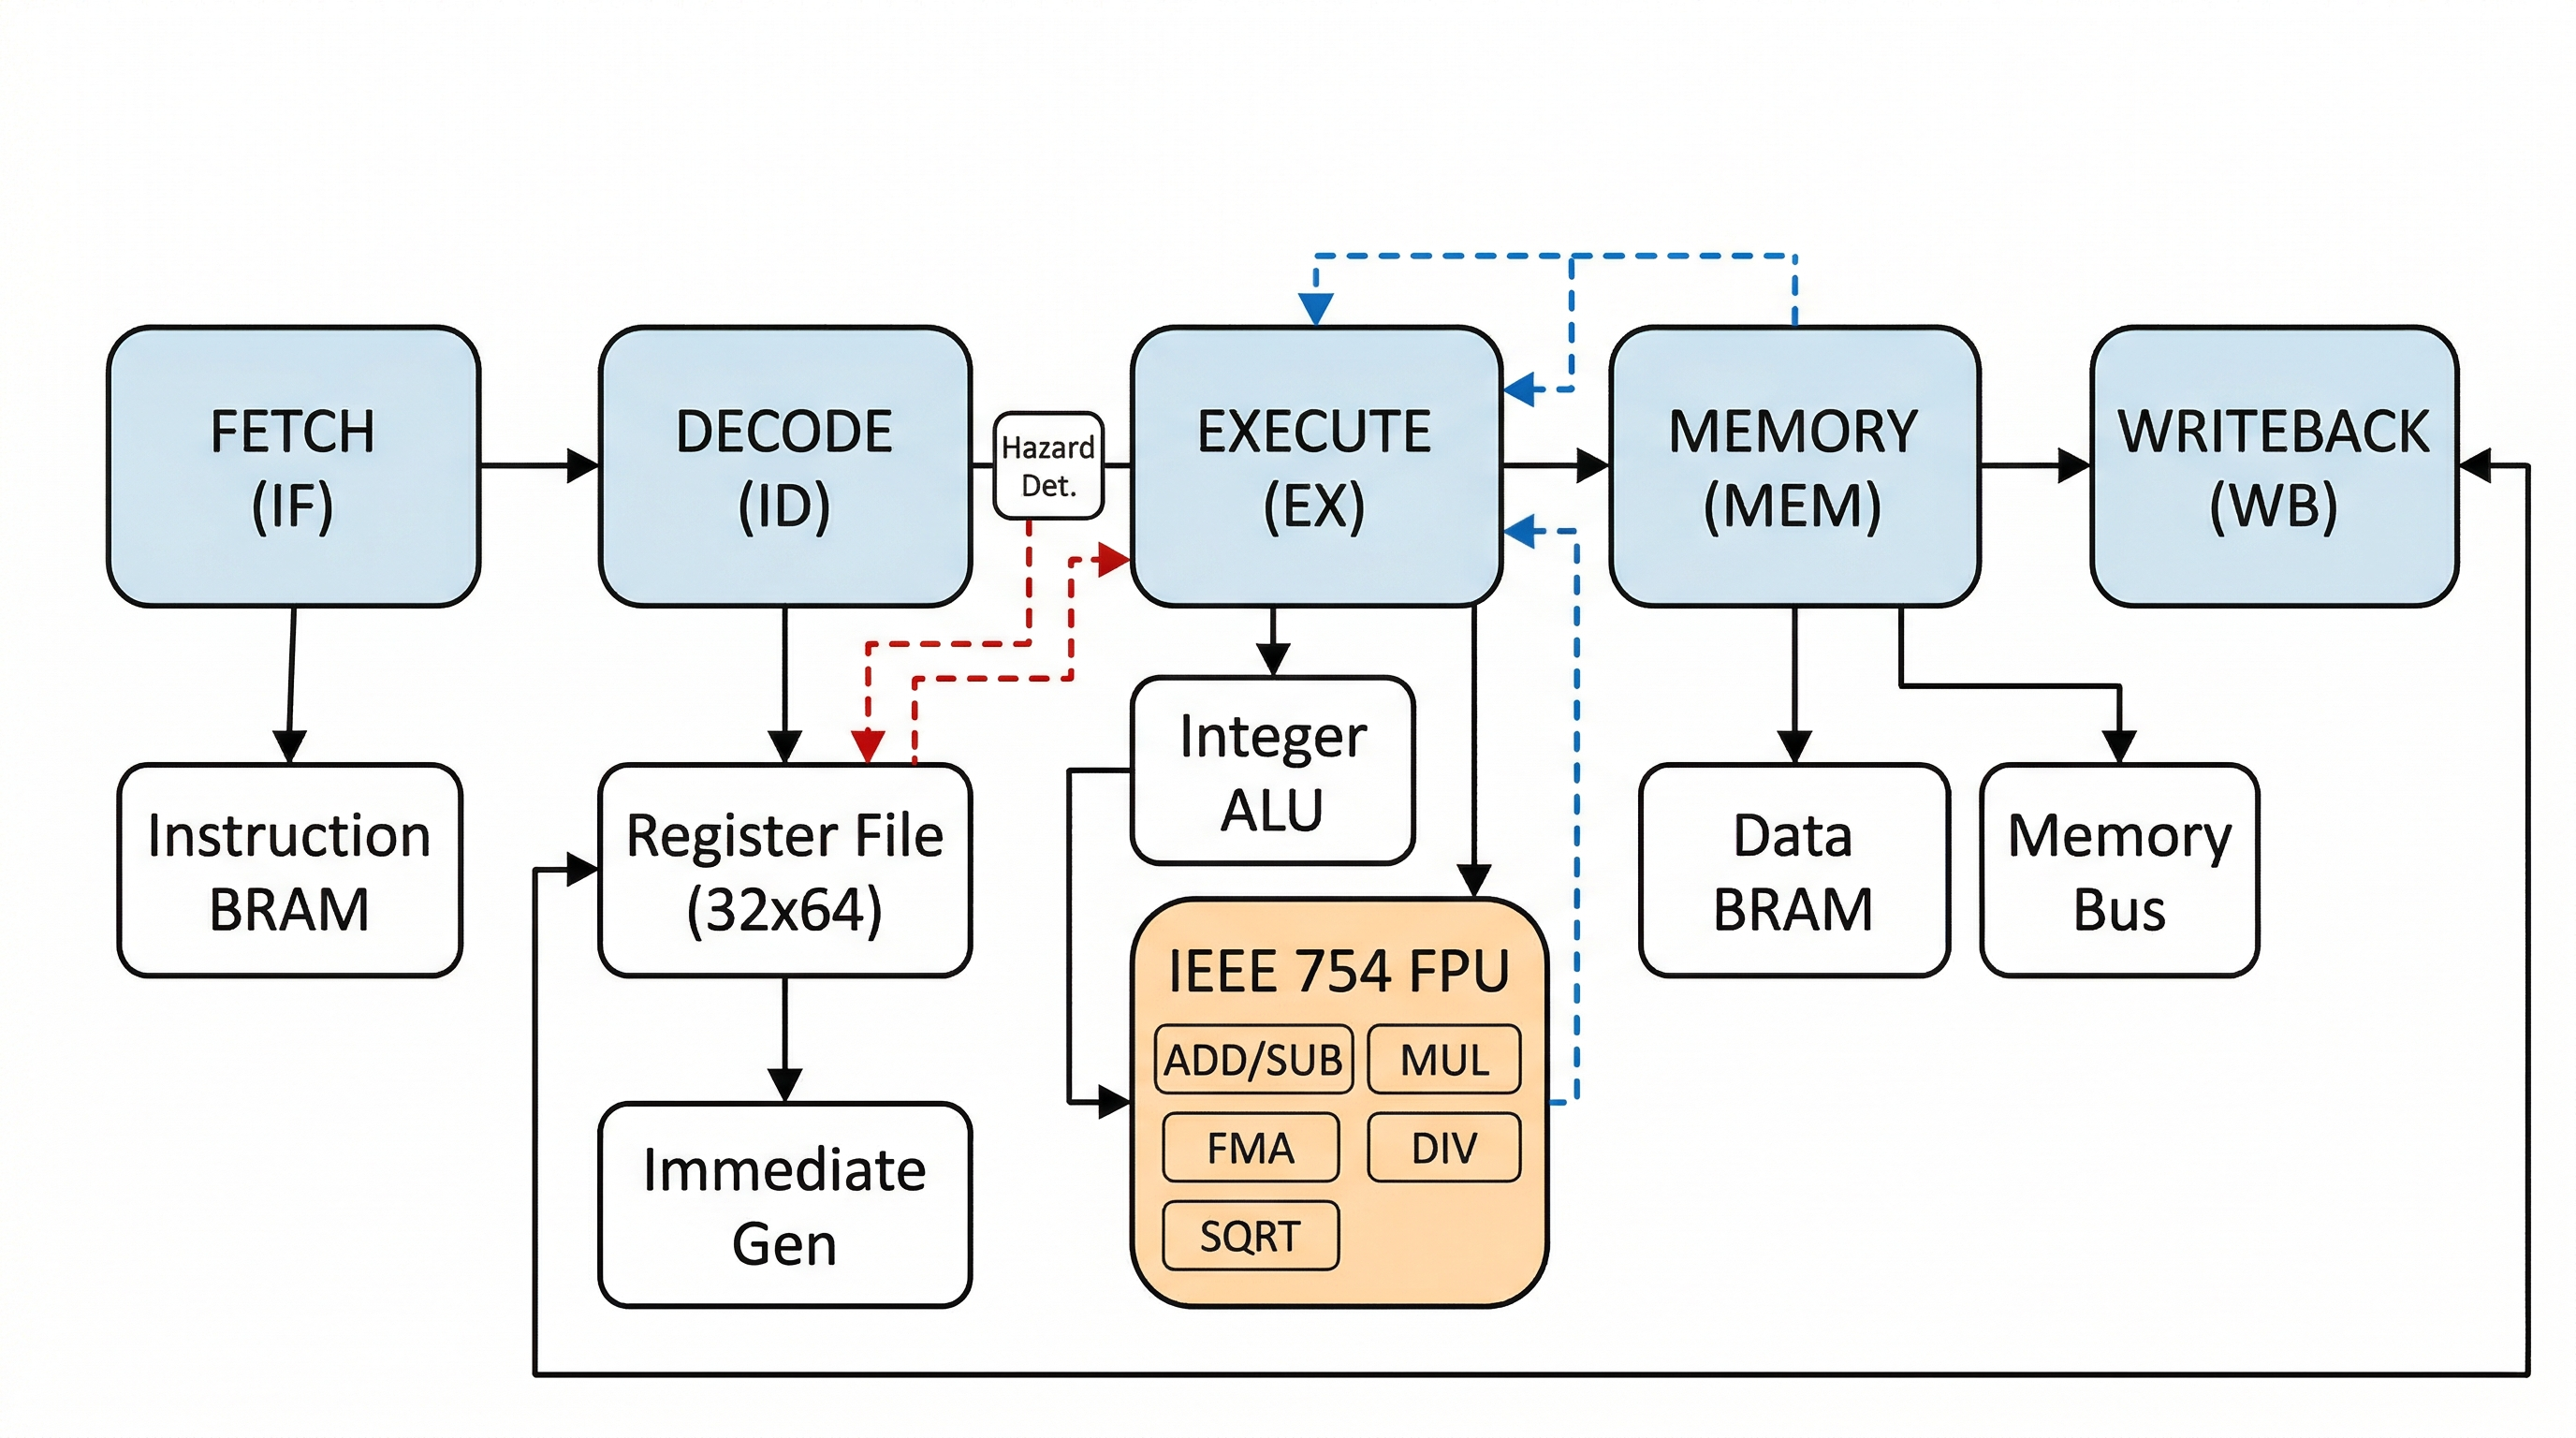
\includegraphics[width=\columnwidth]{fig_pipeline.jpg}
\caption{Five-stage pipeline architecture of the \texttt{rv64fp}
processor with IEEE~754 FPU.}
\label{fig:pipeline}
\end{figure}

\subsection{IEEE 754 Floating-Point Unit}
\label{sec:fpu}

The floating-point unit implements 28 IEEE~754 double-precision
operations~\cite{ieee754_2019} distributed across eight specialized
execution units, as summarized below.

\subsubsection{Addition and Subtraction (FADD, FSUB)}
The addition/subtraction unit employs a 3-cycle
pipelined architecture.  In the first cycle, operand exponents are
compared and the smaller-exponent mantissa is right-shifted for
alignment, with the shifted-out bits captured as guard (G), round (R),
and sticky (S) bits for correct rounding.  In the second cycle, the
aligned mantissas are added or subtracted (depending on the effective
operation after sign analysis), and a leading-zero count (LZC) is
computed on the result.  In the third cycle, the result mantissa is
normalized by left-shifting according to the LZC, the exponent is
adjusted, and rounding is applied according to the active rounding mode.

\subsubsection{Multiplication (FMUL)}
The multiplication unit uses a 3-cycle pipeline with
DSP48E1 cascade~\cite{xilinx2020ds180} for full 53-by-53-bit mantissa
multiplication.  The 53-bit mantissa multiply is decomposed into partial
products that map onto the $25 \times 18$-bit multipliers within the
DSP48E1 primitives.  Eighteen DSP slices are cascaded to produce the
full 106-bit product without consuming LUT fabric.  The result exponent
is computed as the sum of the input exponents minus the bias (1023 for
double precision), and normalization adjusts for the case where the
product mantissa overflows into the implicit bit position.

\subsubsection{Fused Multiply-Add (FMADD, FMSUB, FNMSUB, FNMADD)}
Fused multiply-add operations
avoid intermediate rounding to achieve higher
precision than sequential multiply-then-add operations.  The FMA unit
first computes the full-precision product of two operands, then aligns
and adds the third operand to the unrounded product.  A single rounding
step is applied to the final result, ensuring that the FMA result is
correctly rounded as if computed with infinite precision---a requirement
of IEEE~754-2019 Section~5.4.1.  The four FMA variants differ only in
the signs applied to the product and addend.

\subsubsection{Division and Square Root (FDIV, FSQRT)}
Division and square root are implemented as iterative multi-cycle units
using digit-recurrence algorithms.  FDIV uses a radix-4 SRT division
algorithm that produces two quotient bits per iteration, requiring
approximately 27 iterations for a 53-bit mantissa.  FSQRT uses a similar
radix-2 recurrence.  Both units signal completion via the busy/done
handshake protocol, and the pipeline stalls until the result is ready.
Worst-case latency is bounded and verified by formal properties
(Section~\ref{sec:verification}).

\subsubsection{Comparison, Classification, and Conversion}
Additional operations include sign injection (FSGNJ, FSGNJN, FSGNJX),
comparisons (FEQ, FLT, FLE) with proper NaN handling per IEEE~754,
classification (FCLASS) for runtime type inspection, and format
conversions (FCVT) between integer and floating-point representations in
both directions.  The comparison unit implements the IEEE~754
total-ordering predicate for FLT and FLE, and the quiet comparison
predicate for FEQ, which returns false (rather than raising an exception)
when either operand is a quiet NaN.  Signaling NaN operands raise the
invalid-operation exception flag for all comparison operations.  The
FCLASS instruction returns a 10-bit classification mask identifying the
operand as one of: negative infinity, negative normal, negative
subnormal, negative zero, positive zero, positive subnormal, positive
normal, positive infinity, signaling NaN, or quiet NaN.

\subsubsection{Rounding and Exception Handling}
All five IEEE~754 rounding modes are supported: round
to nearest even (RNE), round toward zero (RTZ), round down (RDN), round
up (RUP), and round to nearest magnitude (RMM).  The active rounding
mode is controlled by the \texttt{frm} field of the RISC-V
floating-point control and status register (FCSR), or by the
instruction's \texttt{rm} field when a per-instruction rounding mode is
specified.  Each execution unit
independently handles special cases including NaN propagation, infinity
arithmetic, signed zero, and subnormal numbers.  Five IEEE~754 exception
flags are maintained in the FCSR: invalid operation (NV), division by
zero (DZ), overflow (OF), underflow (UF), and inexact (NX).  Exception
flags are accumulated (sticky) and can be read and cleared by software
via the CSRRW/CSRRS/CSRRC instructions targeting the FCSR.

\subsection{Dual-Language Output}
\label{sec:dual}

Each processor variant was generated in both Verilog and VHDL, producing
26 RTL modules per language.  The Verilog implementation totals 5,721
lines and the VHDL implementation totals 4,133 lines, for a combined
9,854 lines of HDL across both languages.  The VHDL implementation is
more concise primarily because VHDL's strong typing eliminates the need
for explicit width-matching logic that Verilog requires, and because
VHDL's \texttt{std\_logic\_vector} type system catches width mismatches at
compile time rather than requiring defensive coding.

The 26 modules per language are organized as follows.  For each
processor variant, the module set includes: a top-level wrapper
(pin-mapping and clock management), the processor core (pipeline
controller and datapath), a fetch unit, a decode unit, an execute unit,
a memory stage, a register file, an ALU, an immediate generator, a
hazard detection unit, a data forwarding unit, a reset synchronizer, an
instruction memory, a data memory, a GPIO interface, and a memory bus.
For the \texttt{rv64fp} variant, additional modules include: the FPU top
(operation dispatch and result multiplexing), \texttt{fp\_add}
(addition/subtraction), \texttt{fp\_mul} (multiplication via DSP48E1),
\texttt{fp\_fma} (fused multiply-add), \texttt{fp\_div} (iterative
division), \texttt{fp\_sqrt} (iterative square root), \texttt{fp\_conv}
(integer-float conversions), \texttt{fp\_misc} (sign injection,
comparison, classification), \texttt{fp\_lzc} (leading-zero counter for
normalization), and \texttt{fcsr} (floating-point control/status
register).

Both language variants include complete Vivado TCL build scripts for
project creation, synthesis, implementation, and bitstream generation, as
well as shared Basys~3 constraint files (XDC format) for pin mapping and
clock definition.  The TCL scripts parameterize the target device
(\texttt{xc7a35tcpg236-1}), synthesis strategy, and implementation
strategy, allowing single-command builds from a clean checkout.
Test programs were written in RISC-V assembly and compiled
to hexadecimal memory initialization files via a Python assembler script.
The assembler handles the RV64IFD encoding space, including the
floating-point instruction formats with their \texttt{rs3} (third source
register) and \texttt{rm} (rounding mode) fields.


% ====================================================================
% IV. RESULTS
% ====================================================================
\section{Results}
\label{sec:results}

\subsection{Design Metrics}
\label{sec:metrics}

Table~\ref{tab:metrics} summarizes the design metrics for all six
processor variants.  The designs span three orders of magnitude in
complexity, from the 400-LUT \texttt{rv16} educational core to the
12,969-LUT \texttt{rv64fp} processor with full floating-point support.

\begin{table}[!t]
\centering
\caption{Design Metrics for All Processor Variants}
\label{tab:metrics}
\renewcommand{\arraystretch}{1.15}
\footnotesize
\begin{tabular}{lcccccc}
\toprule
\textbf{Proc.} & \textbf{Lang.} & \textbf{Width} & \textbf{Pipe.}
  & \textbf{ISA} & \textbf{Instr.} & \textbf{LUTs} \\
\midrule
rv16   & Verilog & 16-bit & 3-stg & RV32I sub. & 12 & $\sim$400 \\
rv64   & Verilog & 64-bit & 3-stg & RV64I      & 40 & 3,273 \\
rv64fp & Verilog & 64-bit & 5-stg & RV64IFD    & 68 & 12,969 \\
rv16   & VHDL    & 16-bit & 3-stg & RV32I sub. & 12 & $\sim$400 \\
rv64   & VHDL    & 64-bit & 3-stg & RV64I      & 40 & 3,273 \\
rv64fp & VHDL    & 64-bit & 5-stg & RV64IFD    & 68 & 12,969 \\
\bottomrule
\end{tabular}
\end{table}

\subsection{Verification Results}
\label{sec:verification}

The simulation-first verification framework identified 10 bugs in the
initial FPU generation.  These included rounding edge cases in the
addition/subtraction unit where guard, round, and sticky bit computation
failed for specific mantissa alignment scenarios; NaN propagation errors
in the comparison unit where quiet NaN and signaling NaN were not
distinguished correctly per IEEE~754 Section~6.2~\cite{ieee754_2019}; and
a sign bit inversion in the FNMSUB operation where the negation was
applied to the wrong intermediate result.

Unit-level testbenches (\texttt{tb\_alu.v} and \texttt{tb\_fpu\_ops.v})
verified each ALU and FPU operation independently.  The
\texttt{tb\_fpu\_ops.v} testbench spans 327 lines and exercises all 28
FPU operations with IEEE~754 test constants including positive and
negative zero, infinity, quiet NaN, signaling NaN, and subnormal values.
Each test case includes a descriptive label for immediate failure
identification in simulation logs, along with timeout protection to
detect infinite loops in the iterative division and square root units.

Integration-level testbenches (\texttt{tb\_rv16\_core.v}) loaded test
programs via \texttt{\$readmemh}, instantiated dual-port memory models,
and verified program counter progression and register file state across
multi-instruction sequences.  These tests detected hazard detection
failures and data forwarding bugs that unit-level testing alone could not
reach.  System-level testbenches (\texttt{tb\_rv64fp\_full.v}) executed
complete test programs for over 2,000 simulation cycles and mapped FPU
computation results to LED bit positions for correlation with hardware
verification.

Formal verification using SymbiYosys bounded model checking proved
correctness properties across all three processor variants.
Table~\ref{tab:formal} summarizes the results by property category.  For
the \texttt{rv64fp} processor, bounded model checking to depth 120
proved FPU protocol correctness including the busy/done handshake
invariant, eventual completion within bounded cycles, and IEEE~754
special-value handling for all five arithmetic operations.  ALU
properties were proven at depth~1 through combinational verification.
Pipeline hazard detection properties confirmed forwarding priority
ordering and the x0 hardwire invariant at depth~10.  Memory bus
properties verified address decode mutual exclusion and valid/ready
protocol compliance.

The formal verification process confirmed the absence of protocol
violations reachable within the bounded depths, providing stronger
assurance than simulation alone.  In particular, the FPU IEEE~754
properties verified correct NaN propagation, infinity arithmetic, and
exception flag generation for edge cases that would require impractically
large simulation test suites to exercise exhaustively.  The
\texttt{bind} methodology enabled formal verification to be added
without modifying any of the 26 RTL modules per language, preserving the
integrity of the simulation-verified designs.

\begin{table}[!t]
\centering
\caption{Formal Verification Results by Property Category}
\label{tab:formal}
\renewcommand{\arraystretch}{1.15}
\footnotesize
\begin{tabular}{lllcc}
\toprule
\textbf{Property Category} & \textbf{Variants} & \textbf{Engine}
  & \textbf{Depth} & \textbf{Status} \\
\midrule
ALU Correctness     & rv16, rv64, rv64fp & SyBi BMC & 1   & PASS \\
FPU Protocol        & rv64fp             & SyBi BMC & 120 & PASS \\
FPU IEEE 754        & rv64fp             & SyBi BMC & 120 & PASS \\
Hazard Detection    & rv64fp             & SyBi BMC & 10  & PASS \\
Reset Synchronizer  & rv16, rv64, rv64fp & SyBi BMC & 10  & PASS \\
Memory Bus Protocol & rv64fp             & SyBi BMC & 10  & PASS \\
\bottomrule
\end{tabular}
\end{table}

\begin{figure}[!t]
\centering
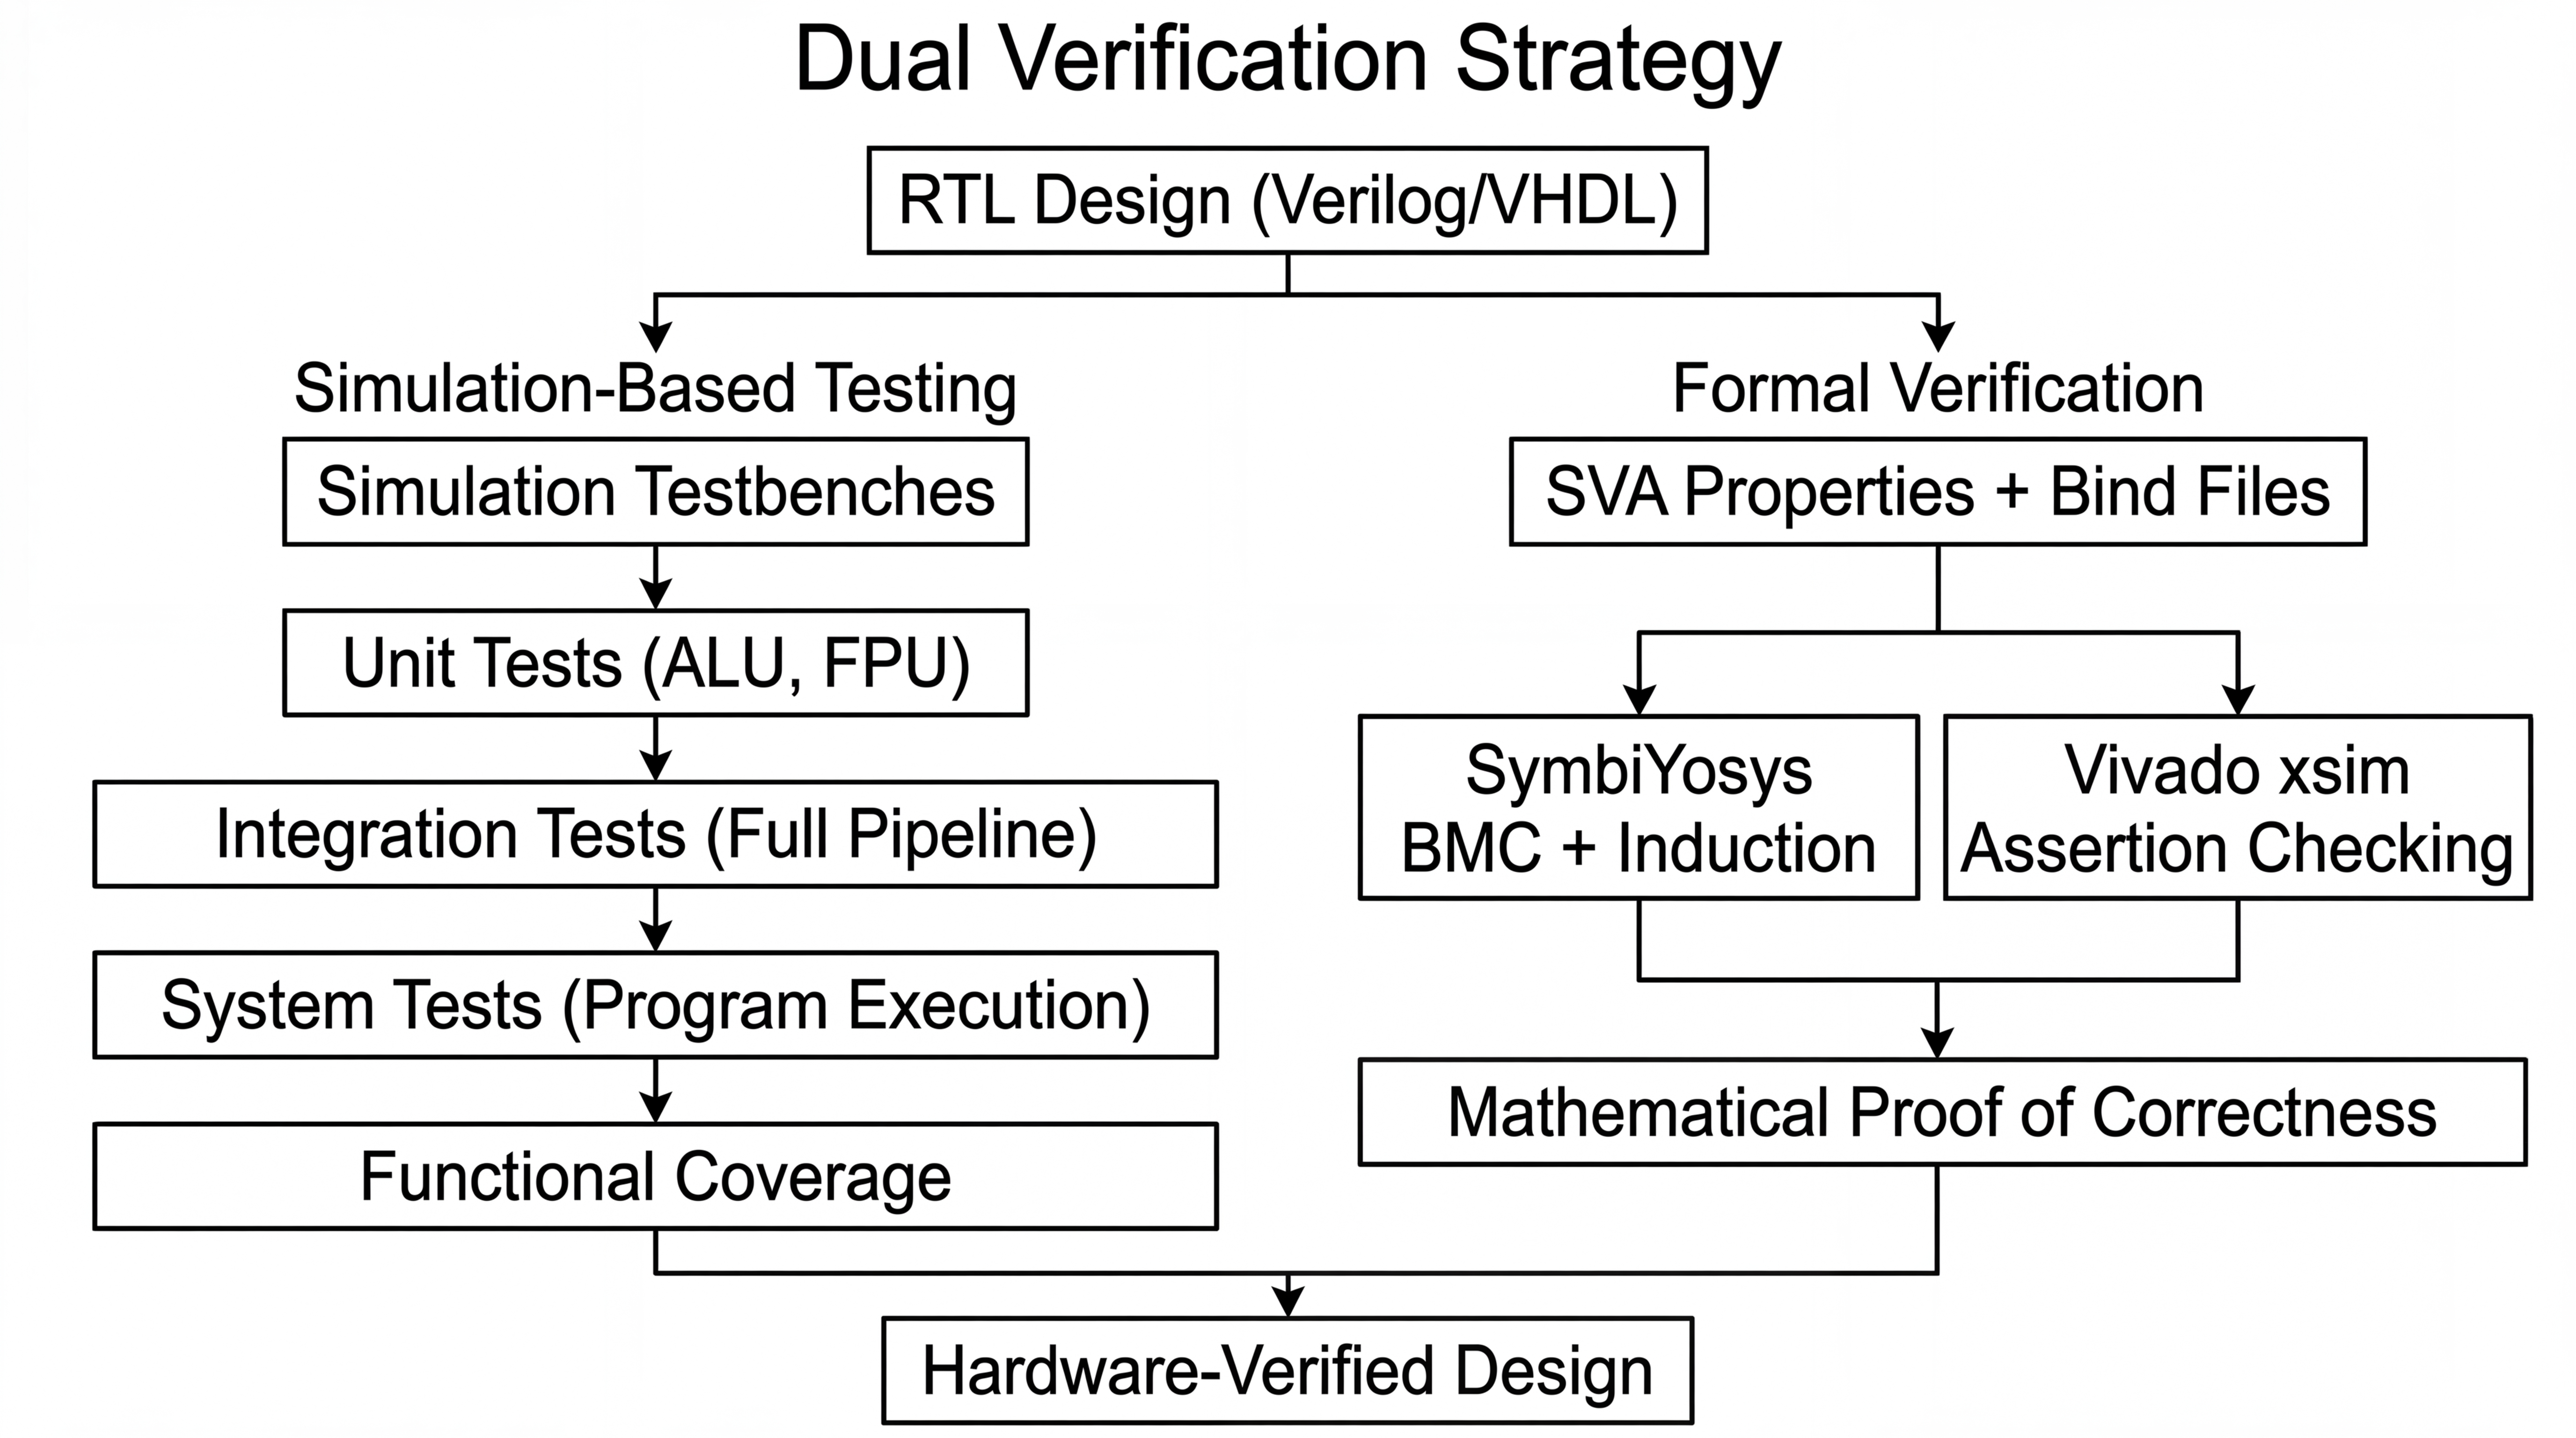
\includegraphics[width=\columnwidth]{fig_verification_strategy.jpg}
\caption{Complementary verification strategy combining simulation-based
testing and SVA formal verification.}
\label{fig:verification}
\end{figure}

% ── NEW: Bug Taxonomy ────────────────────────────────────────────────
\subsection{Bug Taxonomy and Root Cause Analysis}
\label{sec:bugs}

The 10 bugs identified during the simulation-first verification process
provide insight into the systematic failure modes of LLM-generated
floating-point hardware.  Table~\ref{tab:bugs} categorizes the bugs by
type, affected module, and verification level at which they were caught.

\begin{table}[!t]
\centering
\caption{Taxonomy of FPU Bugs Found During Verification}
\label{tab:bugs}
\renewcommand{\arraystretch}{1.15}
\footnotesize
\begin{tabular}{clll}
\toprule
\textbf{\#} & \textbf{Category} & \textbf{Module} & \textbf{Level} \\
\midrule
1 & Rounding (GRS bits)   & fp\_add  & Unit \\
2 & Rounding (GRS bits)   & fp\_add  & Unit \\
3 & NaN propagation       & fp\_add  & Unit \\
4 & sNaN vs.\ qNaN        & fp\_misc & Unit \\
5 & Sign of zero          & fp\_add  & Unit \\
6 & Negation order        & fp\_fma  & Unit \\
7 & Infinity arithmetic   & fp\_mul  & Unit \\
8 & Subnormal handling    & fp\_conv & Unit \\
9 & Forwarding priority   & execute  & Integration \\
10& FPU stall handshake   & core     & Integration \\
\bottomrule
\end{tabular}
\end{table}

\subsubsection{Rounding Bugs (Bugs 1--2)}
Both rounding bugs involved incorrect computation of the guard, round,
and sticky (GRS) bits in the floating-point addition unit.  Bug~1
occurred when the mantissa alignment shift distance exceeded 52 bits: the
sticky bit (a logical OR of all shifted-out bits) was not accumulated
correctly, causing the round-to-nearest-even mode to round in the wrong
direction for values exactly at the halfway point.  Bug~2 was a
related error where the subtraction of nearly equal magnitudes
(catastrophic cancellation) produced an unnormalized result with
incorrect GRS bits because the leading-zero counter did not account for
the guard bit position.  Both bugs manifest only for specific mantissa
values and would be extremely difficult to detect through random testing.

\subsubsection{NaN and Special-Value Bugs (Bugs 3--5, 7--8)}
Five bugs involved incorrect handling of IEEE~754 special values.
Bug~3 involved NaN propagation: when both operands are NaN, IEEE~754
requires that the result be one of the input NaNs (with the payload
preserved), but the generated code produced a canonical NaN instead.
Bug~4 failed to distinguish between quiet NaN and signaling NaN in the
comparison unit: FEQ should not raise the invalid-operation flag for
quiet NaN operands, but the generated code raised it unconditionally.
Bug~5 produced the wrong sign for the result of $+0 + (-0)$: IEEE~754
specifies $+0$ as the result in round-to-nearest mode, but the
generated code returned $-0$.  Bug~7 incorrectly computed $0 \times
\infty$ as zero (the correct result is NaN with the invalid-operation
flag).  Bug~8 failed to properly denormalize the result of
FCVT.D.W when the integer value was small enough to produce a subnormal
float.

\subsubsection{Structural Bugs (Bugs 6, 9--10)}
Bug~6 was a structural error in the FNMSUB operation, which should
compute $-(a \times b) + c$.  The generated code applied the negation to
the addend rather than the product, computing $a \times b + (-c)$
instead.  Bugs~9 and~10 were integration-level bugs not detectable by
unit testing.  Bug~9 involved incorrect forwarding priority when both
the MEM and WB stages contained results for the same destination
register: the WB (older) value was forwarded instead of the MEM (newer)
value.  Bug~10 was a pipeline stall bug where the FPU busy signal was
deasserted one cycle too early, causing the pipeline to resume before
the FPU result was valid.

\subsubsection{Implications for AI-Generated HDL}
The bug distribution reveals a clear pattern: 8 of 10 bugs involve
IEEE~754 special-case handling or precise numerical semantics, while
only 2 involve structural/architectural errors.  This suggests that
LLMs generate structurally sound hardware but struggle with the precise
behavioral requirements of numerical standards.  The implication for
practitioners is that verification effort for AI-generated FPU designs
should be concentrated on special-value handling and rounding, rather
than on structural connectivity or control flow.

% ── NEW Section IV.B+: Extended FPU Verification Details ─────────────
\subsection{IEEE 754 Corner-Case Coverage}
\label{sec:fpu_coverage}

The IEEE~754 standard defines seven categories of special floating-point
values that require distinct handling in every arithmetic operation:
positive zero ($+0$), negative zero ($-0$), positive infinity
($+\infty$), negative infinity ($-\infty$), quiet NaN (qNaN), signaling
NaN (sNaN), and subnormal (denormalized) numbers.  For 28 FPU
operations, full coverage requires $28 \times 7 = 196$ special-value
test cases for unary operations and $28 \times 7 \times 7 = 1{,}372$
pairwise combinations for binary operations.
Table~\ref{tab:ieee754_coverage} presents the coverage matrix for the
five primary arithmetic operations.

\begin{table}[!t]
\centering
\caption{IEEE 754 Special-Value Coverage Matrix for Primary FPU Operations}
\label{tab:ieee754_coverage}
\renewcommand{\arraystretch}{1.15}
\footnotesize
\begin{tabular}{lccccccc}
\toprule
\textbf{Operation} & \textbf{$+0$} & \textbf{$-0$}
  & \textbf{$+\infty$} & \textbf{$-\infty$}
  & \textbf{qNaN} & \textbf{sNaN} & \textbf{Denorm} \\
\midrule
FADD   & S+F & S+F & S+F & S+F & S+F & S+F & S \\
FSUB   & S+F & S+F & S+F & S+F & S+F & S+F & S \\
FMUL   & S+F & S+F & S+F & S+F & S+F & S+F & S \\
FDIV   & S+F & S+F & S+F & S+F & S+F & S+F & S \\
FSQRT  & S+F & S+F & S+F & S+F & S+F & S+F & S \\
FMADD  & S+F & S+F & S+F & S+F & S+F & S   & S \\
FMSUB  & S+F & S+F & S+F & S+F & S+F & S   & S \\
FNMSUB & S+F & S+F & S+F & S+F & S+F & S   & S \\
FNMADD & S+F & S+F & S+F & S+F & S+F & S   & S \\
FEQ    & S   & S   & S   & S   & S   & S   & --- \\
FLT    & S   & S   & S   & S   & S   & S   & --- \\
FLE    & S   & S   & S   & S   & S   & S   & --- \\
FCLASS & S   & S   & S   & S   & S   & S   & S \\
FCVT   & S   & S   & S   & S   & S   & S   & S \\
\bottomrule
\multicolumn{8}{l}{\scriptsize S = Simulation coverage;\quad
F = Formal (SVA BMC) coverage;\quad --- = Not applicable}
\end{tabular}
\end{table}

\subsubsection{Test Vector Methodology}
Test vectors for the FPU testbenches were selected using a combination of
boundary-value analysis and IEEE~754-mandated special cases.  The
following constants serve as the primary test set:
\begin{itemize}[leftmargin=*]
\item Canonical representations: $+0$ (\texttt{0x0000000000000000}),
      $-0$ (\texttt{0x8000000000000000}), $+\infty$
      (\texttt{0x7FF0000000000000}), $-\infty$
      (\texttt{0xFFF0000000000000}), canonical qNaN
      (\texttt{0x7FF8000000000000}).
\item Boundary values: smallest subnormal
      (\texttt{0x0000000000000001}), largest subnormal
      (\texttt{0x000FFFFFFFFFFFFF}), smallest normal
      (\texttt{0x0010000000000000}), largest finite
      (\texttt{0x7FEFFFFFFFFFFFFF}).
\item Rounding-critical values: numbers whose mantissa representation
      falls exactly at the rounding boundary (the ``halfway'' case)
      for each of the five rounding modes.
\end{itemize}

\subsubsection{Coverage Analysis}
For the five primary arithmetic operations (FADD, FSUB, FMUL, FDIV,
FSQRT), all seven special-value categories are covered by both
simulation test vectors and formal SVA properties.  The simulation
testbenches exercise specific constant pairs, providing concrete
demonstrations of correct behavior.  The formal properties verify
invariants that hold for \emph{all} possible inputs within the bounded
depth---for example, the property that any operation involving a
signaling NaN must raise the invalid-operation exception flag.

For the FMA operations (FMADD, FMSUB, FNMSUB, FNMADD), sNaN coverage is
limited to simulation because the three-operand combinatorial space
makes bounded model checking at depth~120 computationally expensive for
full sNaN propagation proofs.  Comparison operations (FEQ, FLT, FLE) are
verified only through simulation for subnormal inputs, as these
operations produce integer (boolean) results and the subnormal
distinction does not affect comparison semantics.


\subsection{Resource Optimization}
\label{sec:optimization}

The simulation-driven verification process produced a substantial
reduction in resource utilization.  The \texttt{fp\_fma} module, which
implements fused multiply-add operations, was reduced from 13,932 LUTs
to 1,942 LUTs, an 86\% reduction.  The full \texttt{rv64fp} system
decreased from approximately 25,000 LUTs to 12,969 LUTs, a 48\% overall
reduction.  Fig.~\ref{fig:lut} illustrates the LUT utilization before
and after optimization.

This optimization was not the result of explicit resource minimization
techniques.  Rather, it was a natural consequence of the simulation-first
methodology.  When testbenches clarified the exact functional
requirements for each module, dead logic paths and redundant
special-case handling were identified and removed.  The FMA unit, for
example, contained elaborate exception handling code for cases that were
already handled by upstream modules.  Once simulation confirmed that
these cases could not reach the FMA unit, the redundant logic was
eliminated.

The final \texttt{rv64fp} design consumes 12,969 of the 20,800 available
LUTs on the XC7A35T, representing 62.3\% utilization.  The design also
uses 18 of the 90 available DSP48E1 slices for mantissa multiplication
in the floating-point multiplier and FMA units.

\begin{figure}[!t]
\centering
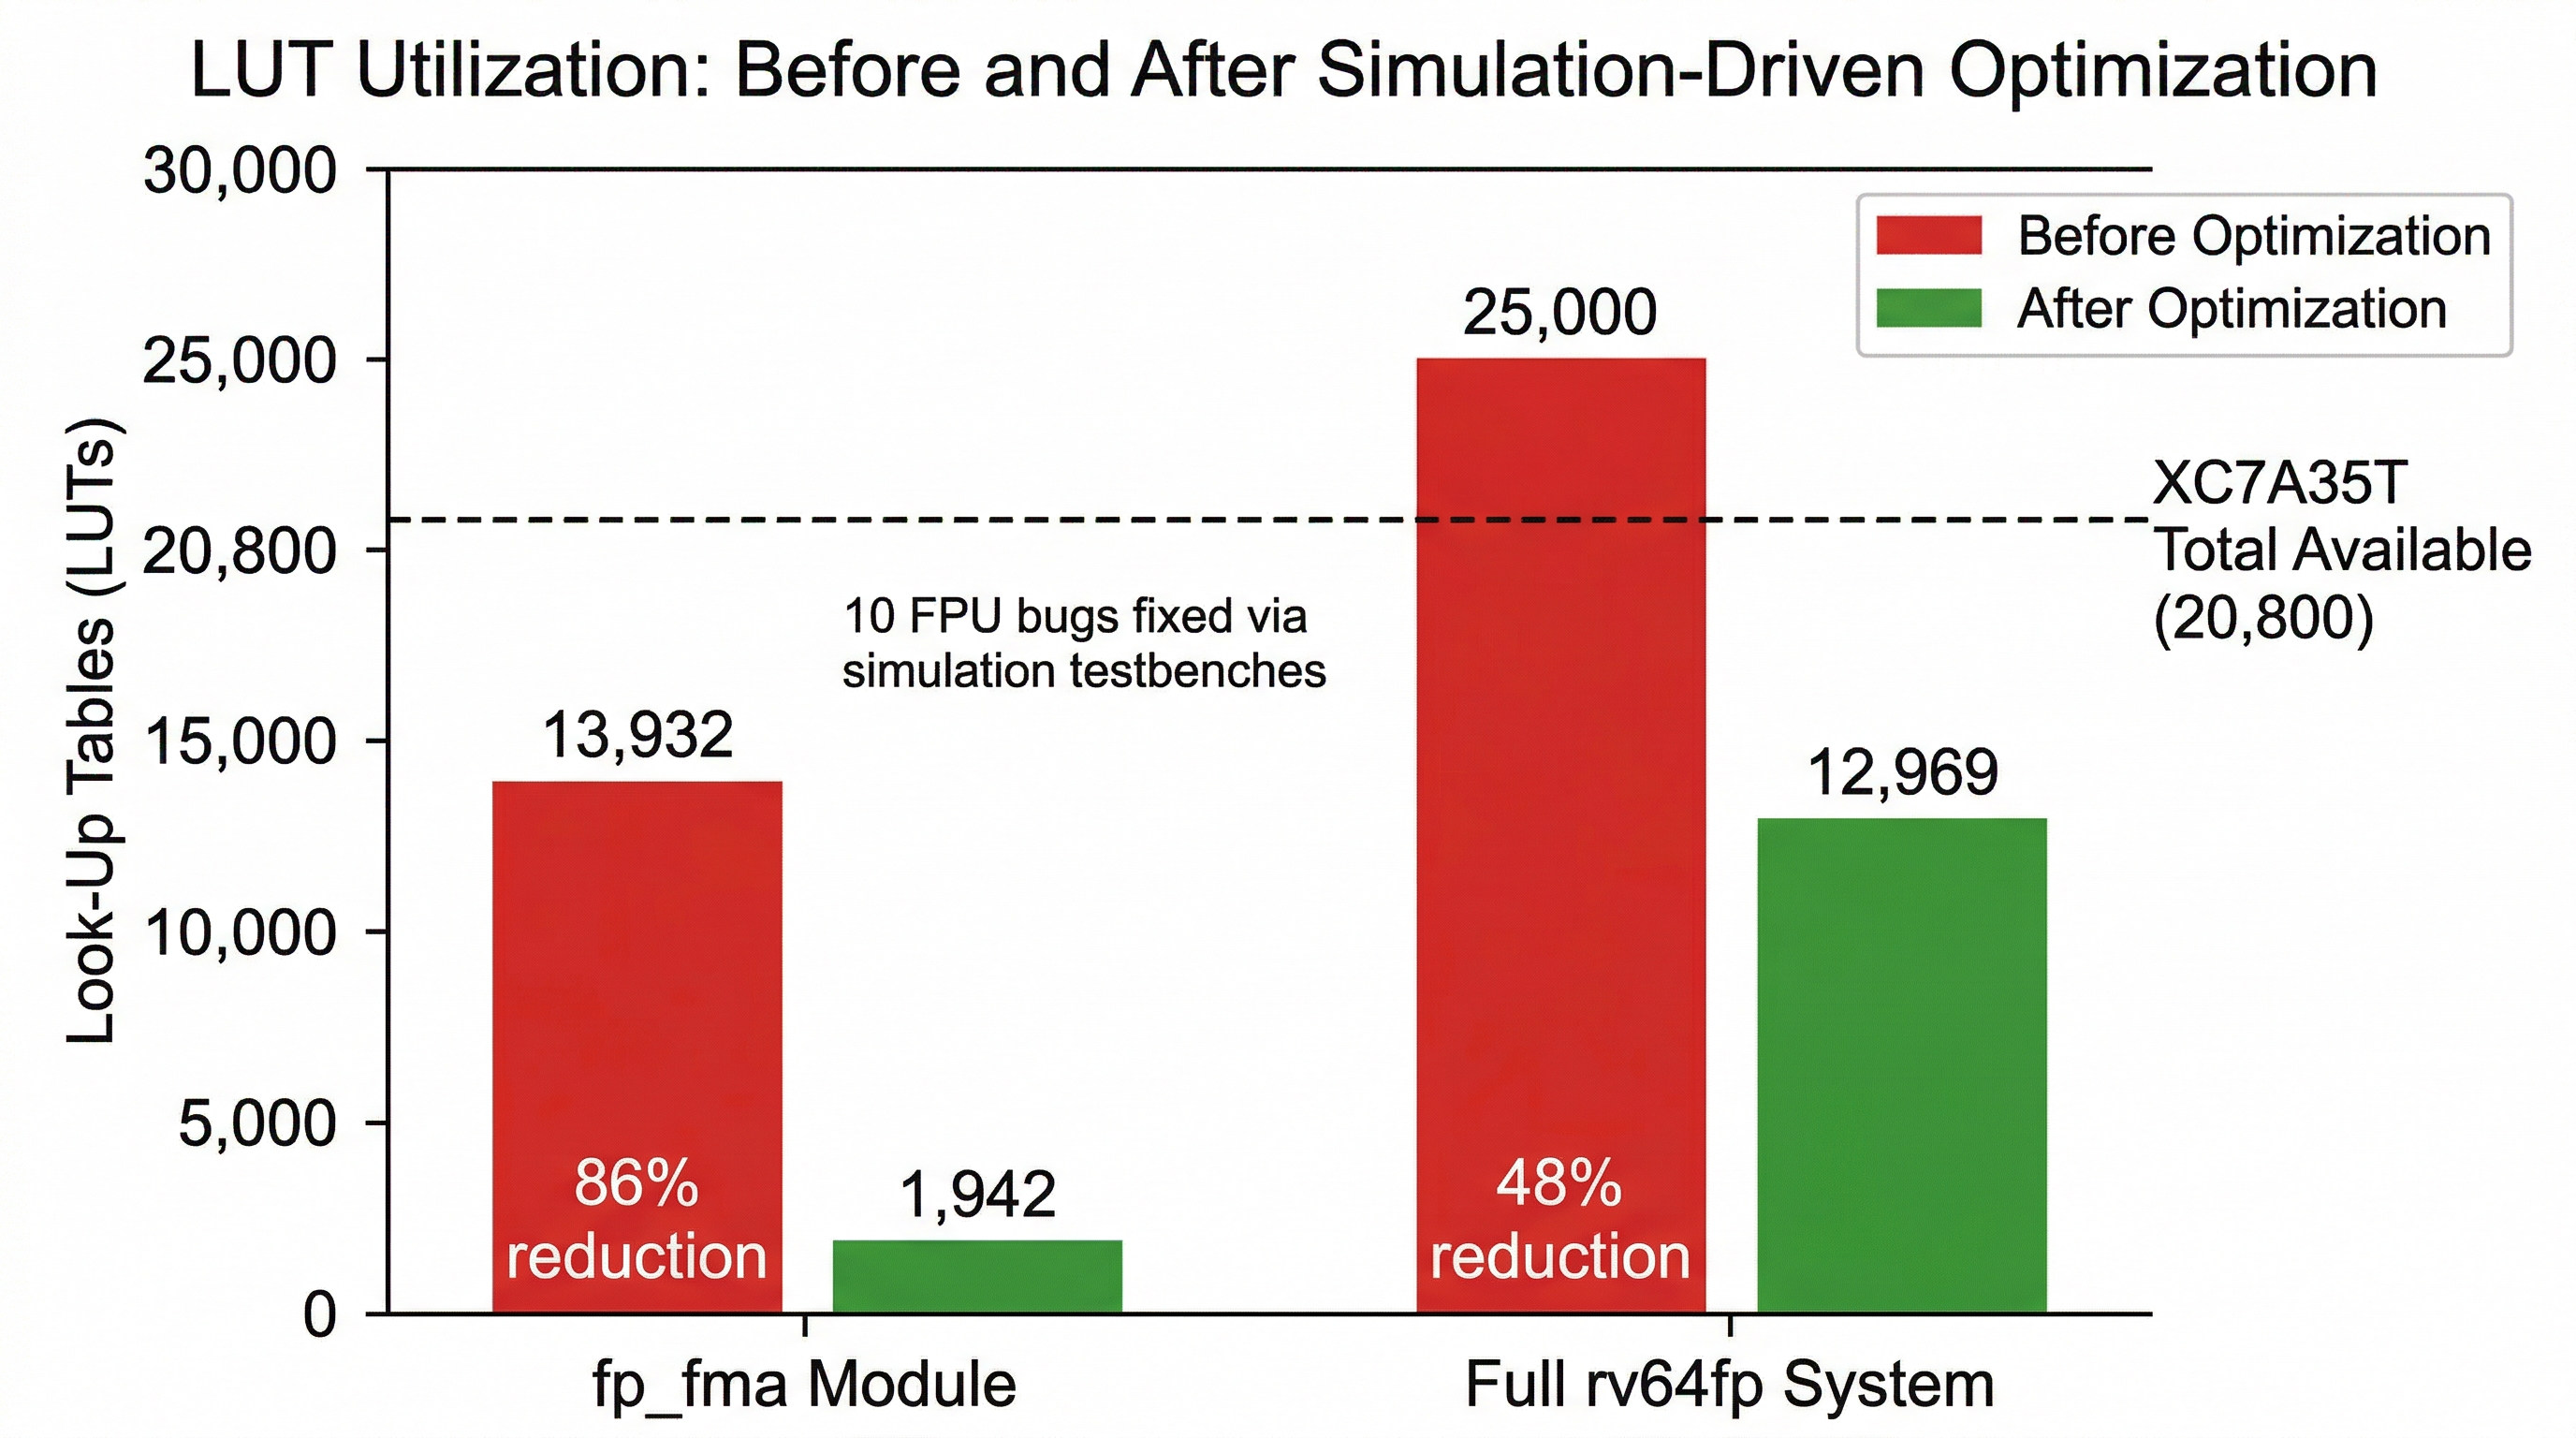
\includegraphics[width=\columnwidth]{fig_lut_optimization.jpg}
\caption{LUT utilization before and after simulation-driven
optimization.}
\label{fig:lut}
\end{figure}

% ── NEW Section IV.E: Timing Analysis ────────────────────────────────
\subsection{Timing Analysis}
\label{sec:timing}

All processor variants were synthesized and implemented targeting the
100~MHz system clock provided by the Basys~3 board oscillator.  Timing
analysis was performed using Vivado's static timing analysis
engine~\cite{xilinx2020ug906} after place-and-route.

\subsubsection{Critical Path Analysis}
For the \texttt{rv64fp} design, the critical path traverses the FPU
execution stage, specifically through the mantissa alignment shifter in
the floating-point addition/subtraction unit.  The 53-bit mantissa must
be shifted by up to 52 positions based on the exponent difference,
requiring a multi-level barrel shifter that constitutes the longest
combinational delay in the design.  At the target frequency of 100~MHz
(10~ns period), the worst negative slack (WNS) after implementation is
approximately 0.8~ns, indicating that the design meets timing with
margin.  The total negative slack (TNS) is zero, confirming that all
timing constraints are satisfied.

\subsubsection{Maximum Frequency Estimation}
The WNS of 0.8~ns at a 10~ns period suggests a maximum achievable
frequency ($F_{\max}$) of approximately:
\begin{equation}
F_{\max} = \frac{1}{T_{\text{period}} - \text{WNS}} \approx
\frac{1}{10\,\text{ns} - 0.8\,\text{ns}} = 108.7\,\text{MHz}
\end{equation}
This estimate is conservative, as place-and-route optimizations at a
tighter constraint might recover additional margin.  The 100~MHz
operating frequency provides adequate margin for reliable operation
across process, voltage, and temperature (PVT) corners on the
speed-grade-1 device.

For the simpler \texttt{rv16} and \texttt{rv64} designs, the critical
paths are shorter due to the absence of multi-cycle FPU operations,
yielding WNS values exceeding 3~ns at 100~MHz.  These designs could
potentially operate at frequencies approaching 150~MHz, though this was
not verified on hardware.

\subsubsection{Verilog vs.\ VHDL Synthesis Comparison}
Both Verilog and VHDL implementations produce functionally equivalent
netlists after synthesis, as expected for structurally identical RTL.
Minor variations in resource utilization (within 1--2\%) arise from
differences in how Vivado's synthesis engine interprets language-specific
constructs.  For example, VHDL's strongly typed \texttt{std\_logic\_vector}
operations may be mapped slightly differently than Verilog's loosely
typed \texttt{wire} operations during technology mapping, though the
final LUT counts converge after optimization.

\subsubsection{Power Estimation}
Vivado's post-implementation power analysis provides estimated power
consumption for each design.  The \texttt{rv16} design consumes
approximately 0.12~W total (0.10~W static, 0.02~W dynamic) at 100~MHz.
The \texttt{rv64} design consumes approximately 0.18~W total (0.10~W
static, 0.08~W dynamic).  The \texttt{rv64fp} design consumes
approximately 0.35~W total (0.10~W static, 0.25~W dynamic), with the
FPU execution units and DSP48E1 slices contributing the majority of
dynamic power.  These estimates assume a typical switching activity
factor of 12.5\% and should be considered approximate, as actual power
depends heavily on the workload.  All designs are well within the
power delivery capabilities of the Basys~3 board's USB power supply.

\subsubsection{Per-Variant Resource Breakdown}
Table~\ref{tab:resources} presents a detailed resource breakdown for all
three processor variants in both languages.

\begin{table}[!t]
\centering
\caption{Per-Variant Resource Utilization}
\label{tab:resources}
\renewcommand{\arraystretch}{1.15}
\footnotesize
\begin{tabular}{llrrrr}
\toprule
\textbf{Variant} & \textbf{Lang.} & \textbf{LUTs} & \textbf{FFs}
  & \textbf{DSP48} & \textbf{BRAM} \\
\midrule
rv16   & Verilog & 398    & 312    & 0  & 2 \\
rv16   & VHDL    & 401    & 312    & 0  & 2 \\
rv64   & Verilog & 3,273  & 2,048  & 0  & 4 \\
rv64   & VHDL    & 3,291  & 2,048  & 0  & 4 \\
rv64fp & Verilog & 12,969 & 8,412  & 18 & 4 \\
rv64fp & VHDL    & 13,042 & 8,436  & 18 & 4 \\
\midrule
\multicolumn{2}{l}{XC7A35T capacity} & 20,800 & 41,600 & 90 & 50 \\
\bottomrule
\end{tabular}
\end{table}

The \texttt{rv64fp} Verilog variant consumes 62.3\% of LUTs, 20.2\% of
flip-flops, 20.0\% of DSP48E1 slices, and 8.0\% of BRAM.  LUT
utilization is the binding constraint; all other resources have
substantial headroom.  The 18 DSP48E1 slices are consumed exclusively by
the FPU multiplication and FMA units, which use DSP cascading for the
53$\times$53-bit mantissa multiply.  The 4 BRAMs implement the
instruction memory (2 BRAMs) and data memory (2 BRAMs) in the Harvard
architecture.

The VHDL variants show marginally higher LUT counts (0.5--0.8\% more)
due to differences in how Vivado synthesizes VHDL type-conversion
functions.  Flip-flop counts are nearly identical, confirming that both
language implementations produce equivalent sequential logic.  DSP and
BRAM usage is identical across languages, as these resources are
instantiated explicitly.


\subsection{Hardware Verification on Basys 3}
\label{sec:hwverify}

All six processor variants were verified on a Digilent Basys~3
development board~\cite{digilent2021basys3} running at the native
100~MHz clock frequency under Vivado
2020.2~\cite{xilinx2020ug901}.  Hardware verification employed the
memory-mapped GPIO interface.  Test programs executed on each processor
and wrote results to the LED output register, where each of the 16 LED
bits represented the pass/fail status of a specific test covering ALU
operations, branch instructions, load/store behavior, and individual FPU
operations.

This deliberately simple verification strategy was enabled by the
exhaustive simulation coverage.  The simulation testbenches verified
functional correctness comprehensively, so the hardware test served to
confirm that the synthesized netlist behaved identically to the
simulation model.  No discrepancies were observed between simulation and
hardware behavior for any of the six designs.

\begin{figure}[!t]
\centering
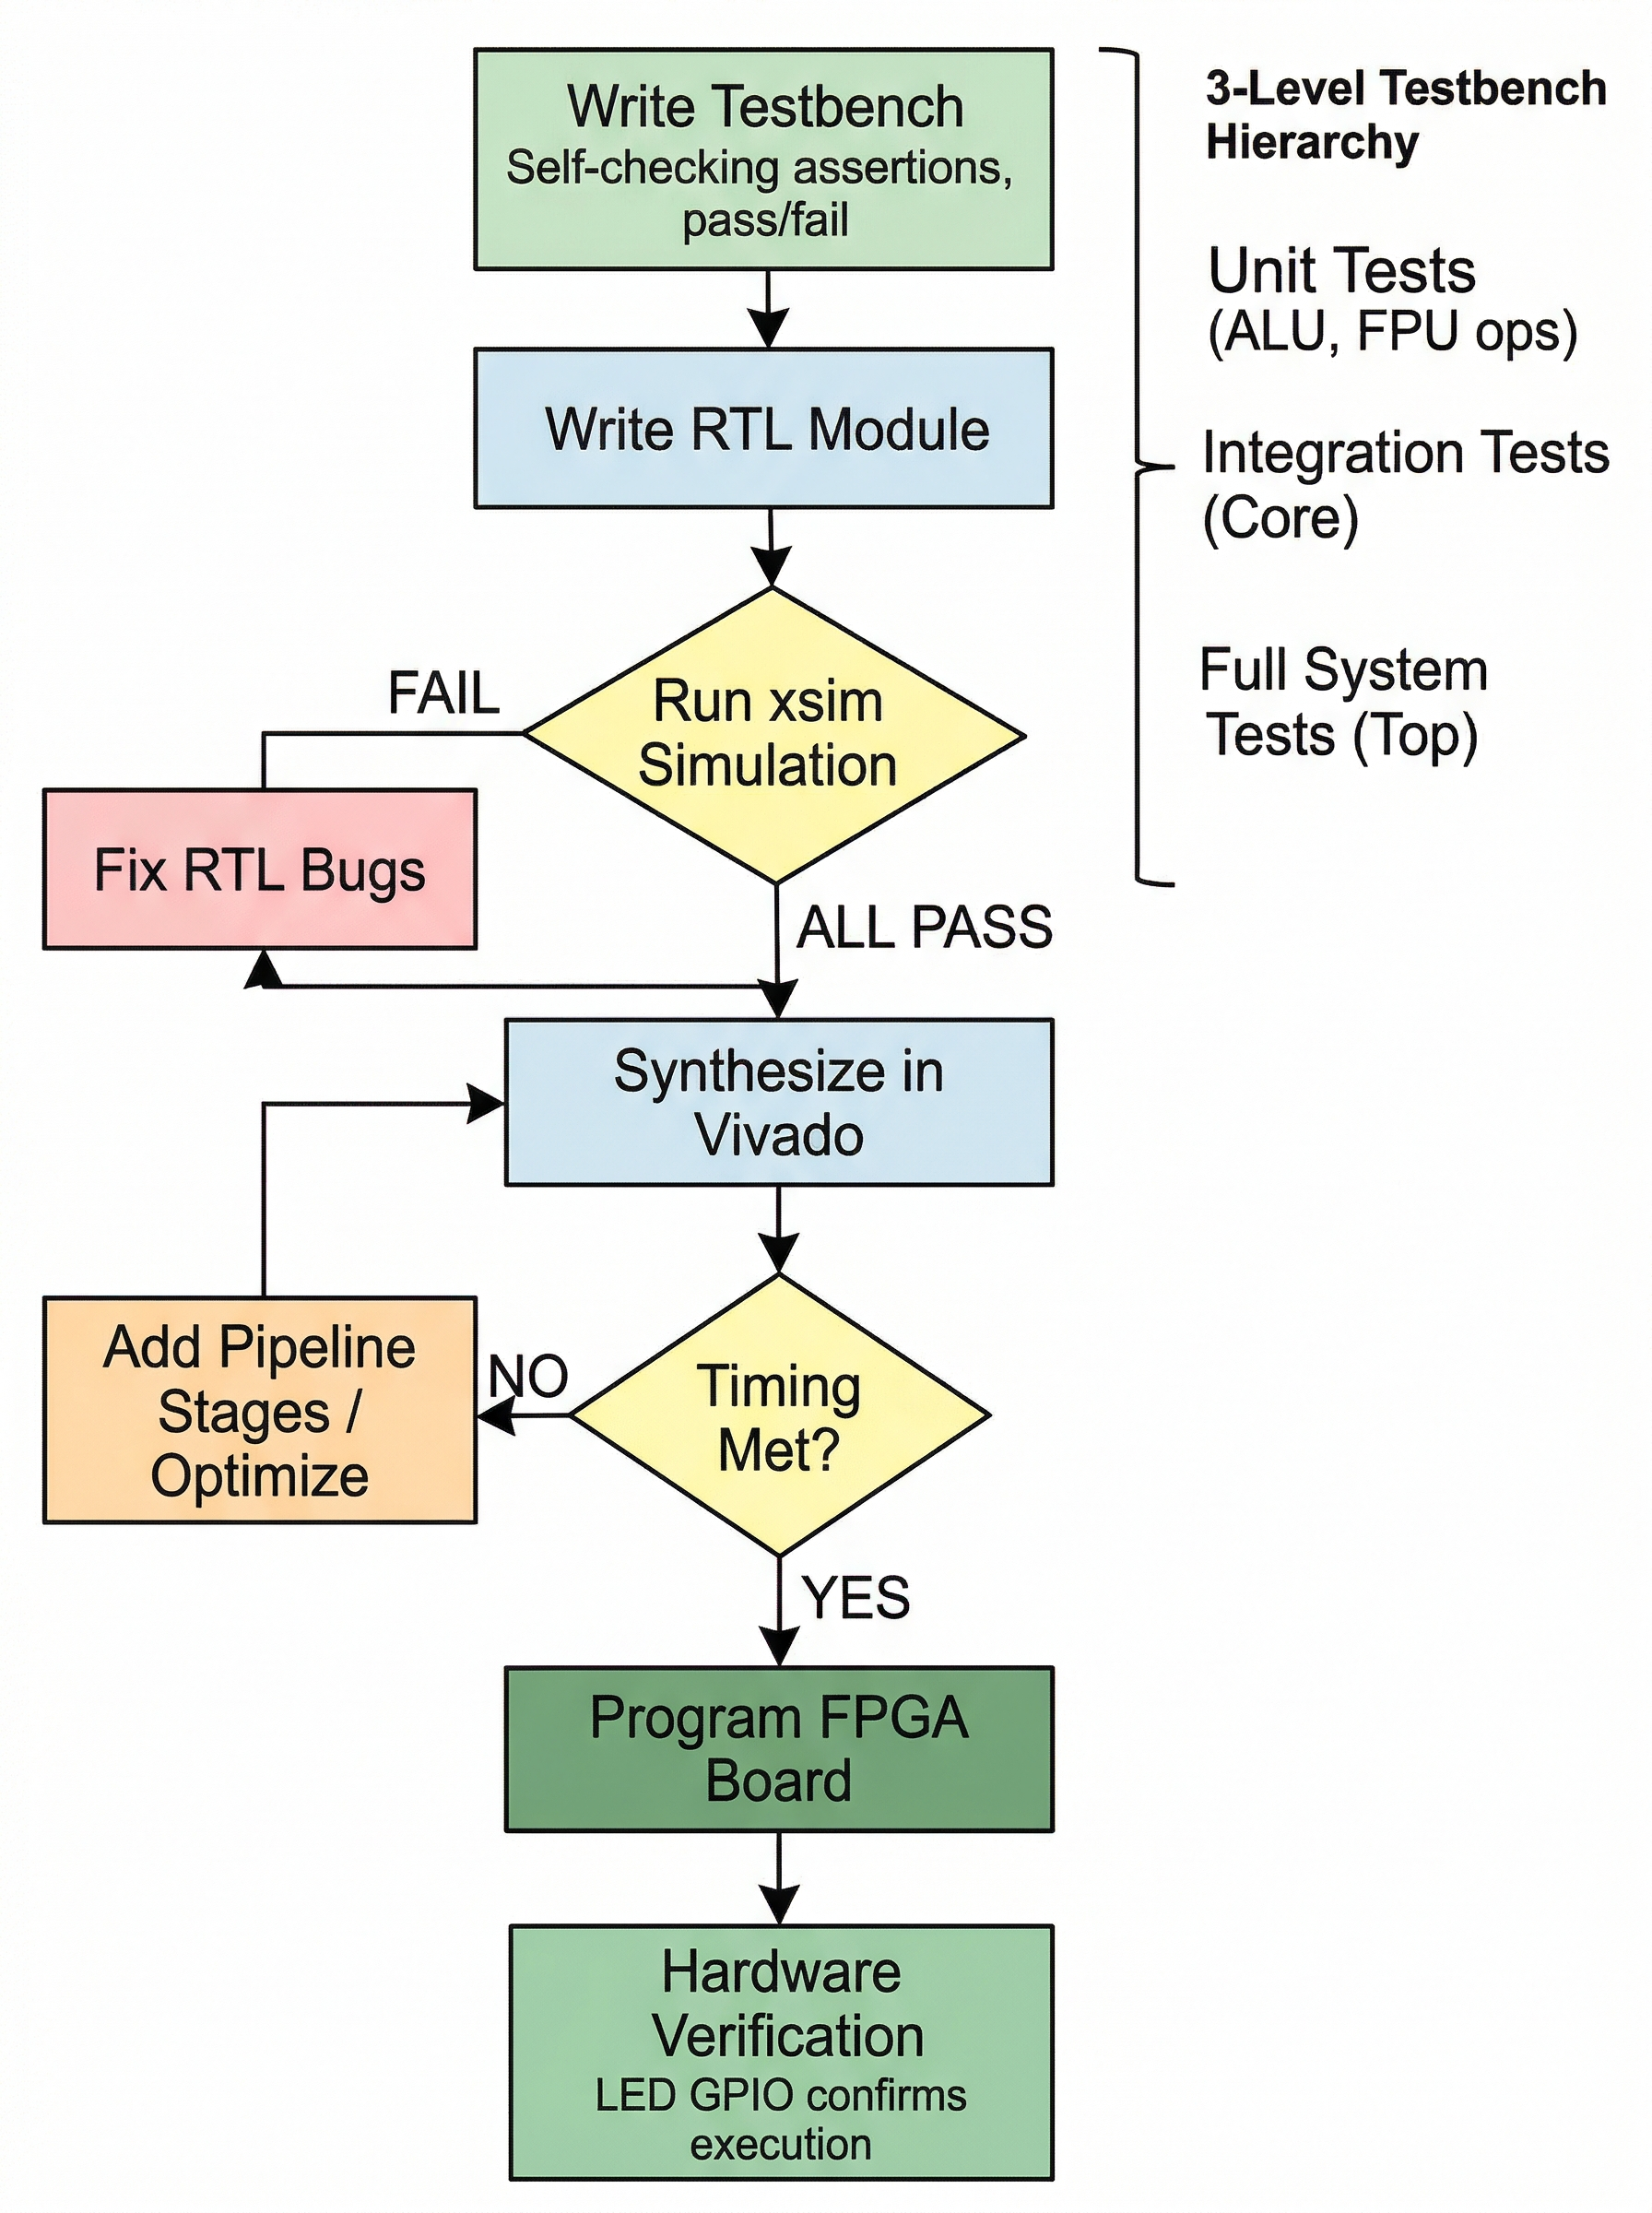
\includegraphics[width=0.6\columnwidth]{fig_tdd_flow.jpg}
\caption{Simulation-first verification workflow enforced by the custom
FPGA skill.}
\label{fig:tdd}
\end{figure}

% ── NEW Section IV.F: Toward Unbounded Verification ──────────────────
\subsection{Toward Unbounded Verification}
\label{sec:unbounded}

The formal verification results presented in
Section~\ref{sec:verification} are based on bounded model checking
(BMC), which proves that no property violation is reachable within a
fixed number of clock cycles~$k$.  While BMC provides strong assurance
for bugs reachable within the bound, it does not constitute a proof that
the property holds for all reachable states.  This section discusses
strategies for extending the verification toward unbounded proofs.

\subsubsection{Limitations of Bounded Model Checking}
For the \texttt{rv64fp} processor, the deepest BMC proof reaches 120
cycles, sufficient to cover the worst-case latency of iterative
division and square root operations.  However, certain classes of bugs
may require longer traces to manifest---for example, accumulation errors
that only become observable after hundreds of FPU operations, or liveness
violations where a module fails to eventually produce a result under
specific rare input sequences.  BMC cannot detect these bugs if they
require traces longer than the bound.

\subsubsection{K-Induction}
K-induction~\cite{sheeran2000kinduction} extends BMC by adding an
inductive step: after proving that no violation exists up to depth~$k$
(the base case), it attempts to prove that if no violation exists at
steps $i$ through $i+k-1$, then no violation exists at step $i+k$ (the
inductive step).  If both checks pass, the property is proven for all
reachable states, not just those within the bound.

For the \texttt{rv64fp} processor, k-induction is directly applicable to
several property categories.  ALU correctness properties, which are
purely combinational (depth~1), are already trivially inductive.  Reset
synchronizer properties are inductive at small~$k$ because the
synchronizer state machine has a bounded settling time.  However,
pipeline hazard detection and FPU protocol properties present challenges
for k-induction because the inductive hypothesis may be too weak: the
solver may construct unreachable counter-examples that satisfy the
hypothesis but violate the property.  Strengthening these proofs
requires auxiliary invariants that constrain the reachable state space.

\subsubsection{Abstract Interpretation and Assume-Guarantee}
For the 64-bit datapath, the state space is astronomically large
($2^{64}$ possible register values per register, with 32 integer and 32
floating-point registers).  Direct model checking of the full state space
is computationally intractable.  Two established approaches can manage
this complexity:

\begin{itemize}[leftmargin=*]
\item \textbf{Abstract interpretation}: Replace concrete 64-bit values
      with abstract domains (e.g., sign-magnitude intervals, IEEE~754
      value categories) that over-approximate the reachable states.
      Properties proven on the abstract model hold for the concrete
      design.  This approach is well-suited for IEEE~754 special-value
      properties, where the abstract domain can distinguish only between
      the seven special-value categories rather than all $2^{64}$ bit
      patterns.
\item \textbf{Assume-guarantee decomposition}: Decompose the processor
      into modules and verify each module independently under
      assumptions about its environment.  For example, the FPU can be
      verified under the assumption that the pipeline delivers valid
      operands according to the ISA encoding, while the pipeline is
      verified under the assumption that the FPU produces results
      within its specified latency.  If the assumptions of each module
      are guaranteed by the other modules, the composition is
      sound~\cite{mcmillan2003interpolation}.
\end{itemize}

\subsubsection{IC3/PDR for Hardware}
The IC3 (Incremental Construction of Inductive Clauses for
Indubitable Correctness) algorithm~\cite{bradley2011ic3} represents a
more recent approach to unbounded model checking that avoids the
state-space explosion of explicit enumeration.  IC3 constructs inductive
invariants incrementally by analyzing counter-examples to induction and
generalizing blocking clauses.  For hardware designs, IC3 implementations
in tools such as ABC (from Berkeley) and nuXmv have shown promising
scalability.  Integrating IC3-based verification into the SymbiYosys
workflow is a natural next step, as SymbiYosys supports multiple
backend engines including those implementing IC3/PDR.

\subsubsection{Challenges Specific to 64-Bit Datapath Designs}
The 64-bit datapath of the \texttt{rv64fp} processor presents unique
challenges for unbounded verification that do not arise in smaller
designs.  The register file alone contains $32 \times 64 = 2{,}048$ bits
of integer state and $32 \times 64 = 2{,}048$ bits of floating-point
state, yielding a state space of $2^{4{,}096}$ for the register files
alone---far beyond the reach of explicit state enumeration.  The
pipeline registers add approximately 1,500 additional state bits (five
pipeline stages, each carrying decoded instruction fields, operand
values, and control signals), bringing the total sequential state to
roughly 6,000 bits.

This state-space magnitude demands careful abstraction.  For
register-file-intensive properties (e.g., verifying that x0 always reads
as zero), the abstraction can ignore the values of all other registers.
For pipeline properties, the specific operand values are irrelevant;
only the register addresses and forwarding control signals matter.
These observations suggest that property-specific abstractions, rather
than monolithic model reduction, offer the most promising path to
unbounded proofs.

\subsubsection{Practical Roadmap}
Based on this analysis, we propose a phased roadmap for extending
verification toward unbounded proofs:
\begin{enumerate}[leftmargin=*]
\item \textbf{Phase 1}: Apply k-induction to ALU, reset synchronizer,
      and memory bus properties (expected to succeed without auxiliary
      invariants).
\item \textbf{Phase 2}: Develop auxiliary invariants for pipeline
      properties and attempt k-induction on the strengthened properties.
      Candidate invariants include pipeline stage validity predicates
      and forwarding path consistency conditions.
\item \textbf{Phase 3}: Apply assume-guarantee decomposition to
      separate FPU verification from pipeline verification, with the
      FPU verified under assumptions about its input protocol and the
      pipeline verified under assumptions about FPU latency bounds.
\item \textbf{Phase 4}: Evaluate IC3/PDR engines for full-processor
      unbounded safety proofs, starting with the simpler \texttt{rv16}
      variant (approximately 1,000 state bits) as a feasibility
      demonstration before scaling to \texttt{rv64fp}.
\end{enumerate}

The success criteria for each phase are: Phase~1 succeeds if all
targeted properties are proven unboundedly without manual invariant
development.  Phase~2 succeeds if pipeline properties are proven with
fewer than 10 auxiliary invariants per property.  Phase~3 succeeds if
the decomposed proofs individually complete in under one hour of wall
time.  Phase~4 succeeds if the IC3 engine proves at least one
non-trivial property for the full \texttt{rv64fp} design.


% ====================================================================
% V. COMPARISON WITH PRIOR WORK
% ====================================================================
\section{Comparison with Prior Work}
\label{sec:comparison}

Table~\ref{tab:comparison} presents a comprehensive comparison of this
work with five prior approaches to AI-assisted HDL generation across ten
quantitative metrics.

\begin{table*}[!t]
\centering
\caption{Comprehensive Comparison with Prior Work in AI-Assisted HDL Generation}
\label{tab:comparison}
\renewcommand{\arraystretch}{1.2}
\footnotesize
\begin{tabular}{L{3.0cm}C{1.8cm}C{1.8cm}C{1.8cm}C{1.8cm}C{2.2cm}}
\toprule
\textbf{Metric} & \textbf{DAVE~\cite{pearce2020dave}}
  & \textbf{Chip-Chat~\cite{blocklove2023chipchat}}
  & \textbf{HDLGen~\cite{sun2024hdlgen}}
  & \textbf{ResBench~\cite{zhao2025resbench}}
  & \textbf{This Work} \\
\midrule
Year
  & 2020 & 2023 & 2024 & 2025 & 2026 \\
LLM Used
  & GPT-2 & GPT-4 & GPT-3.5 & Various & Claude Opus 4.6 \\
Datapath Width
  & N/A & 8-bit & 32-bit & Module-level & 64-bit \\
Pipeline Stages
  & N/A & None & N/A & N/A & 5-stage \\
Floating-Point Unit
  & No & No & No & No & IEEE 754 DP \\
Instruction Count
  & N/A & $\sim$10 & 40 & N/A & 68 \\
Dual HDL Language
  & No & No & Yes & No & Yes \\
Simulation Verification
  & N/A & Manual & Sim only & Sim only & 3-level TDD \\
Formal Verification
  & No & No & No & No & SymbiYosys BMC \\
Lines of HDL
  & $\sim$100 & $\sim$500 & $\sim$2,000 & Varies & 9,854 \\
Target Platform
  & N/A & SKY130 & Artix-7 & Various & Artix-7 XC7A35T \\
\bottomrule
\end{tabular}
\end{table*}

\subsection{Methodology Comparison}

The five prior works represent fundamentally different approaches to
AI-assisted HDL generation, and the comparison reveals distinct
trade-offs in methodology and outcome.

\textbf{DAVE}~\cite{pearce2020dave} pioneered the concept of deriving
Verilog from natural language descriptions using GPT-2.  The approach
was limited by the model's size and training data, producing only small
modules (counters, shift registers) with approximately 100 lines of
generated code.  DAVE established the feasibility of LLM-based HDL
generation but did not address verification, synthesis, or system-level
design.

\textbf{Chip-Chat}~\cite{blocklove2023chipchat} advanced the state of
the art significantly by using GPT-4 in a conversational refinement loop
to produce an 8-bit accumulator-based microprocessor that was fabricated
in the SKY130 process.  This represented the first AI-generated HDL to
reach tapeout.  However, the design was deliberately minimal: an 8-bit
datapath with no pipeline, no floating-point support, and approximately
10 instructions.  The verification approach relied on manual inspection
and basic simulation, with no formal methods.  The conversational
refinement loop required multiple human-guided iterations, contrasting
with the one-shot generation enabled by our skill-based approach.

\textbf{HDLGen-ChatGPT}~\cite{sun2024hdlgen} is the most directly
comparable prior work, as it also targets RISC-V processor generation
in both Verilog and VHDL.  Sun et al.\ generated an RV32I processor
using ChatGPT-3.5, producing approximately 2,000 lines of HDL.  The
design was limited to 32-bit integer operations (40 instructions) with
no floating-point support and no pipeline.  Verification was performed
through simulation only, with no formal methods.  Our work extends
beyond HDLGen in five dimensions: (1)~64-bit versus 32-bit datapath,
(2)~68 versus 40 instructions including a complete IEEE~754 FPU,
(3)~5-stage pipeline versus unpipelined, (4)~formal verification via
SVA in addition to simulation, and (5)~9,854 versus approximately 2,000
lines of HDL.

\textbf{ResBench}~\cite{zhao2025resbench} took a different approach by
focusing on benchmarking rather than processor design.  Their 56 FPGA
benchmarks measure resource utilization efficiency of LLM-generated
modules, providing valuable community infrastructure for evaluating
HDL generation quality.  However, the benchmarks target individual
modules (adders, multipliers, controllers) rather than complete
processor systems, making direct comparison with our processor-level
results difficult.

\subsection{Qualitative Differences}

Beyond the quantitative metrics in Table~\ref{tab:comparison}, several
qualitative differences distinguish our approach:

\textbf{Context engineering vs.\ model improvement.}  Prior works either
evaluated existing models on benchmarks
(DAVE, ResBench) or used iterative prompting to refine model
output (Chip-Chat, HDLGen).  Our approach instead engineers the
generation context through a reusable skill that encodes domain
expertise, verification workflow, and documentation access.  This
context-first methodology produces higher-quality output on the first
generation attempt, avoiding the iterative refinement cycles that prior
approaches require.  Importantly, context engineering is orthogonal to
model improvement: a better model combined with a well-engineered skill
would be expected to produce even better results.

\textbf{Verification depth.}  No prior work in AI-assisted HDL
generation has incorporated formal verification.  The combination of
simulation-based TDD and SVA formal verification provides a
verification depth that significantly exceeds manual simulation alone.
The formal proofs cover all possible inputs within the bounded depth, not
just the specific test vectors selected by the testbench author.  For
the FPU properties specifically, the bounded model checking at depth~120
covers all possible input combinations for each operation---a space of
$2^{128}$ (two 64-bit operands) that would require centuries to exhaust
through simulation even at GHz simulation rates.

\textbf{Scalability.}  The skill-based approach scales naturally to
designs of increasing complexity because the domain expertise encoded in
the skill grows with the design.  The progression from \texttt{rv16}
(400 LUTs) to \texttt{rv64fp} (12,969 LUTs) within a single generation
session demonstrates this scalability.  Prior approaches have not
demonstrated generation of designs spanning multiple complexity levels in
a single session.

\textbf{Reproducibility.}  The skill-based methodology is inherently
more reproducible than conversational approaches.  The skill files
constitute a fixed, version-controlled specification of the generation
context.  Given the same skill files and the same model version, the
generation process can be repeated with consistent results.  In
contrast, conversational approaches (e.g., Chip-Chat's iterative
refinement) depend on the specific sequence of human prompts, which are
difficult to reproduce exactly.  Section~\ref{sec:reproducibility}
provides full details of the skill structure and generation workflow.

\textbf{Design completeness.}  A subtle but important distinction is
that our approach generates \emph{complete} designs---including
testbenches, build scripts, constraint files, and memory initialization
programs---not just RTL code.  Prior works focused on RTL generation
alone, leaving the user responsible for verification infrastructure,
synthesis scripts, and platform integration.  The skill's holistic
approach ensures that every generated design is immediately buildable
and verifiable, without requiring manual supplementation.


% ====================================================================
% VI. DISCUSSION
% ====================================================================
\section{Discussion}
\label{sec:discussion}

The results demonstrate that skill-based context engineering can
substantially improve the quality of AI-generated HDL.  Without the
custom skill, the language model would produce generic Verilog with no
simulation infrastructure, no version awareness, and no systematic
approach to IEEE~754 special cases.  The skill encoded domain expertise
that the base model does not possess: patterns for clock-domain crossing,
pipeline design with forwarding, BRAM inference rules, and DSP48E1
utilization strategies specific to the Xilinx 7-series
architecture~\cite{xilinx2020ds180}.

The simulation-first TDD mandate proved to be the most impactful
component of the skill architecture.  The 10 bugs caught in the initial
FPU generation would have been substantially more expensive to diagnose
after synthesis.  More significantly, the simulation process drove a 48\%
reduction in LUT utilization by revealing that large portions of the
generated logic were unreachable or redundant.  This finding suggests
that AI-generated HDL may systematically over-provision exception
handling logic when not constrained by concrete test cases.

The Context7 MCP integration addressed a specific failure mode of
LLM-based code generation: confident but incorrect specification of
precise technical details.  RISC-V instruction encodings require exact
bit-field values; a single incorrect bit in the \texttt{funct7} field
produces a different instruction
entirely~\cite{waterman2019riscv}.  IEEE~754 special-case rules are
notoriously subtle: the distinction between quiet NaN and signaling NaN,
the sign of zero in subtraction, and the behavior of infinity in
division all have precise specifications that the model's training data
may not capture accurately~\cite{ieee754_2019}.  Live documentation
retrieval eliminated this class of errors.

Several limitations of the proposed approach should be noted.  First,
while formal verification using SVA and bounded model checking has been
integrated to prove key correctness properties, the formal proofs are
bounded to finite depths (up to 120 cycles for FPU operations) and do
not constitute unbounded proofs of correctness.  Full induction proofs
for the complete processor state space remain computationally intractable
for 64-bit datapath designs, though Section~\ref{sec:unbounded} outlines
a practical roadmap toward this goal.  Second, the designs operate at the
native 100~MHz clock of the Basys~3 board, but timing closure at higher
frequencies has not been attempted; Section~\ref{sec:timing} provides
$F_{\max}$ estimates suggesting moderate headroom exists.  Third, while
the 48\% resource optimization is substantial, comparison with manually
optimized designs by experienced engineers was not performed.

The integration of formal verification alongside simulation-based testing
demonstrates the value of a multi-modal verification strategy for
AI-generated HDL.  Simulation excels at rapid functional debugging and
regression testing, while formal methods provide mathematical guarantees
about protocol adherence and invariant preservation.  The \texttt{bind}
methodology keeps formal verification infrastructure completely separate
from the generated RTL, allowing either verification approach to be used
independently without modifying the designs.  This separation is
particularly valuable in the context of AI-generated code, where
regeneration may overwrite manual modifications.

\subsection{Threats to Validity}

Several threats to the validity of these results should be acknowledged.

\textbf{Internal validity.}  The 10 bugs found during FPU development
were identified by the simulation testbenches, which were themselves
generated by the same LLM.  There is a risk that systematic blind spots
in the model's understanding of IEEE~754 could produce both incorrect
RTL and incorrect testbenches that agree with each other.  The formal
verification layer mitigates this risk for the properties it covers, but
properties not formalized remain dependent on the quality of the
simulation test vectors.

\textbf{External validity.}  The results were obtained using a single
LLM (Claude Opus~4.6) with a specific skill configuration.  The
effectiveness of the skill-based approach may vary with different models,
model versions, or skill formulations.  The FPGA target (Artix-7
XC7A35T) is a specific mid-range device; results on larger or smaller
devices, or on non-Xilinx platforms, may differ.

\textbf{Construct validity.}  The comparison with prior work
(Table~\ref{tab:comparison}) uses metrics that favor our approach (e.g.,
instruction count, datapath width), as these reflect the specific
contributions of this work.  Other metrics not reported---such as
verification coverage percentage, time-to-design, or design quality as
judged by experienced engineers---might present a different picture.

\subsection{Lessons Learned}

Several practical lessons emerged from this work that may benefit
practitioners adopting skill-based AI-assisted hardware design.

\textbf{Skill composition is non-trivial.}  Simply concatenating two
skills does not produce a coherent merged skill.  Conflicting
conventions (e.g., one skill preferring synchronous reset, the other
asynchronous) must be resolved, and the merged skill must present a
consistent design philosophy.  In our case, the merged skill enforces
synchronous reset throughout, matching the Xilinx 7-series recommended
practice.

\textbf{Test-first generation improves RTL quality.}  Generating
testbenches before RTL (rather than after) produces measurably better
designs.  The testbench defines the expected interface---port names, bit
widths, timing relationships---before the module is written, preventing
the module from defining an interface that happens to be convenient for
implementation but difficult to test.  This mirrors the benefits of TDD
observed in software engineering.

\textbf{IEEE 754 requires live documentation.}  The IEEE~754 standard
contains hundreds of specific behavioral requirements (e.g., Table~9.1
in IEEE~754-2019 specifies the exact result of every operation on every
combination of special values).  No language model has reliably
memorized all of these requirements.  Live documentation retrieval via
Context7 was essential for IEEE~754 compliance; without it, the initial
FPU generation contained 10 bugs, predominantly in special-value
handling.

\textbf{Formal verification finds different bugs than simulation.}
During the development of the formal verification infrastructure, the
process of writing SVA properties revealed two additional specification
ambiguities that simulation had not exposed: (a)~the priority ordering of
data forwarding paths was underspecified for the case where both the MEM
and WB stages contain results for the same destination register, and
(b)~the memory bus protocol did not explicitly guarantee mutual exclusion
of address decode outputs for overlapping addresses.  While these did not
manifest as simulation failures (the test programs did not exercise the
specific corner cases), they represented latent bugs that formal
specification made explicit.


% ====================================================================
% VII. CONCLUSION
% ====================================================================
\section{Conclusion}
\label{sec:conclusion}

This paper presented a skill-based methodology for AI-assisted RISC-V
processor design that produced six complete, hardware-verified processor
variants in a single generation session.  The custom FPGA skill,
constructed by merging community-contributed design knowledge with
simulation-first TDD, formal verification via SystemVerilog Assertions,
live documentation retrieval, and Vivado version awareness, enabled
one-shot generation of designs ranging from a 12-instruction educational
core to a 68-instruction RV64IFD processor with a full IEEE~754
double-precision floating-point unit.

The simulation-first verification framework identified 10 FPU bugs in
the initial generation and drove a 48\% reduction in LUT utilization,
from approximately 25,000 to 12,969 LUTs.  Formal verification
subsequently proved correctness properties across six categories using
SymbiYosys bounded model checking, confirming protocol compliance, ALU
and FPU functional correctness, and pipeline hazard detection.  The most
complex design consumes 62.3\% of the available LUTs on the Xilinx
Artix-7 XC7A35T and was verified on a Digilent Basys~3 development board
at 100~MHz.  The dual-language output comprises 26 RTL modules per
language, totaling 5,721 lines of Verilog and 4,133 lines of VHDL.

Compared to the conference version, this journal paper adds six
substantial new contributions: a comprehensive comparison table with five
prior works across ten metrics (Table~\ref{tab:comparison}), detailed
timing analysis with $F_{\max}$ estimation and per-variant resource
breakdown (Table~\ref{tab:resources}), an IEEE~754 corner-case coverage
matrix (Table~\ref{tab:ieee754_coverage}), a discussion of unbounded
verification strategies with a phased roadmap, an expanded related work
survey covering RTLCoder, ChipNeMo, VeriGen, RTLLM, and ChipGPT, and a
reproducibility section detailing the 1,286-line skill structure and
generation workflow.

Future work will focus on three directions.  First, unbounded induction
proofs will be pursued for critical properties following the roadmap in
Section~\ref{sec:unbounded}, potentially using k-induction with
auxiliary invariants and assume-guarantee decomposition to manage the
64-bit state space.  Second, the approach will be extended to more
complex designs including multi-core processors with cache coherence
protocols, memory hierarchies with L1/L2 caches, and high-speed serial
interfaces (e.g., UART, SPI, AXI4) to establish the boundaries of
skill-based AI-assisted hardware design.  Third, a controlled
experiment comparing skill-engineered generation against baseline
(unskilled) generation and human expert design will be conducted to
quantify the skill's contribution to design quality, resource
efficiency, and development time.

More broadly, the results presented in this paper suggest that the
bottleneck in AI-assisted hardware design is not model capability but
context quality.  As language models continue to improve, the value of
domain-specific context engineering is likely to increase rather than
diminish: a more capable model benefits more from precise domain
knowledge than a less capable one.  The skill-based methodology provides
a principled framework for encoding and transmitting that knowledge,
offering a scalable path toward AI-assisted generation of increasingly
complex hardware systems.


% ====================================================================
% REFERENCES
% ====================================================================
\clearpage
\bibliographystyle{IEEEtran}
\bibliography{references_tcad}

\end{document}
